\documentclass{report}
\usepackage[utf8]{inputenc}
\usepackage[T1]{fontenc}
\usepackage[french]{babel}
\usepackage{lmodern}
\usepackage{amsmath}
\usepackage{amssymb}
\usepackage{amsthm}
\usepackage{algorithm}
\usepackage{algpseudocode}
\usepackage{array}
\usepackage{pgf,tikz}
\usetikzlibrary{arrows}
\usepackage{pgf,tikz}

\theoremstyle{plain}
\newtheorem{proposition}{Proposition}
\newtheorem{theorem}{Théorème}
\newtheorem{lemma}{Lemme}
\newtheorem{corollary}{Corollaire}


\theoremstyle{definition}
\newtheorem{definition}{Définition}
\newtheorem{conjecture}{Conjecture}

\theoremstyle{remark}
\newtheorem{remark}{Remarque}
\newtheorem{example}{Exemple}
	
\title{Compte-rendu}
\author{Vincent \textsc{Auriau} -- Laurent \textsc{Beaughon} -- Marc \textsc{Belicard} \\ Yaqine \textsc{Hechaichi} -- Thaïs \textsc{Rahoul} -- Pierre \textsc{Vigier}}

\begin{document}

\maketitle

\tableofcontents

\chapter{Réseaux de neurones}

\section{Apprentissage automatique}

Avant de parler de neurones et de réseaux de neurones, nous commencerons par rappeler rapidement ce qu'est l'apprentissage automatique, ses différentes formes et fixerons certaines notations pour la suite de ce document.

L'apprentissage automatique au sens général peut être défini comme un processus permettant à une machine d'évoluer afin de résoudre une tâche ou un problème. Il en existe plusieurs formes parmi lesquelles l'apprentissage supervisé, l'apprentissage non-supervisé et l'apprentissage par renforcement.

L'apprentissage supervisé est celui qui nous intéressera le plus, il sera donc davantage détaillé. Dans un problème d'apprentissage il est donné un ensemble de taille finie $N$ de couples d'entrée, sortie que nous noterons $(x^{(1)},y^{(1)}), ..., (x^{(N)}, y^{(N)})$. Ces couples sont appelés exemples. Les entrées proviennent d'un espace $\mathcal{X}$ de dimension $n$ et les sorties d'un espace $\mathcal{Y}$ de dimension $m$. Une hypothèse classique de l'apprentissage automatique est de supposer que les entrées sont générées de manière indépendante selon une certaine loi de probabilité sur $\mathcal{X}$. Plus formellement, les $(x^{(i)})_{i \in \{1, ..., N\}}$ sont les réalisations de variables aléatoires $(X_i)_{i \in \{1, ..., N\}}$ avec les $X_i$ indépendantes et identiquement distribuées selon une probabilité $p$. Pour plus de commodités, notons $X = \{x^{(i)}, \forall i \in \{1, ..., N\}\}$ et $Y = \{y^{(i)}, \forall i \in \{1, ..., N\}\}$.

L'objectif de l'apprentissage supervisé est alors de découvrir le processus générateur des sorties à partir des entrées. Si ce processus est déterministe, il s'agira d'une fonction $f$ générant les sorties à partir des entrées. L'objectif de l'apprentissage sera donc de trouver à partir des exemples un modèle $\hat{f}$ proche de f. Si le processus est non déterministe, il s'agira alors de retrouver la loi de $p(y|x)$.

Si les sorties prennent leurs valeurs dans un espace $\mathcal{Y}$ infini, le problème est dit de régression. Dans le cas contraire, on parle de problème de classification. Par convention, on choisit les valeurs des classes telles que $\mathcal{Y} = \{0, ..., M-1\}$ avec $M$ le nombre de classes. Si $M = 2$, il s'agit de classification binaire.

Quelque soit le type de problème à résoudre, l'objectif est toujours de trouver une fonction ou une distribution de probabilité proche de celle générant les sorties. Cependant, cette notion de "proche" est très relative. 

\begin{definition}[Erreur sur un exemple]
Soit $e : \mathbb{R}^m \times \mathbb{R}^m \rightarrow \mathbb{R}$ la mesure de performance sur un exemple.
\end{definition}
$e(y, \hat{f}(x))$ représentera l'écart de notre modèle avec la sortie attendue. 

\begin{example}[Erreur quadratique]
Une mesure courante est l'erreur quadratique $e(x, y) \mapsto \Vert x - y \Vert_2^2$.
\end{example}

On définit alors l'erreur sur l'ensemble des exemples :

\begin{definition}[Erreur empirique]
$$
E_{in} = \frac{1}{N}\sum_{i=1}^{N}{e(y^{(i)}, f(x^{(i)})} = \mathbb{E}_{x, y \sim \hat{p}_{data}}(e(y, f(x)))
$$
avec $\hat{p}_{data}$ est la distribution empirique dans l'ensemble des exemples.
\end{definition}

Et l'erreur dans l'absolue, sur toutes les valeurs possibles :

\begin{definition}[Erreur absolue]
$$
E_{out} = \mathbb{E}_{x, y \sim p}(e(y, f(x)))
$$
avec $p$ la distribution réelle des entrées et des sorties.
\end{definition}

L'objectif d'être proche peut alors se traduire par la minimisation de $E_{out}$. Or l'estimation de $E_{out}$ nécessite de connaître $p(x, y)$ pour tout $(x, y)$ dans $\mathcal{X} \times \mathcal{Y}$, ce qui est généralement impossible. Cependant, il est aisé de calculer $E_{in}$, qui est une estimation de $E_{out}$ sur les données disponibles. 

En effet, on a la proposition suivante :
\begin{proposition}
$E_{in}$ est un estimateur non biaisé de $E_{out}$.
\end{proposition}

\begin{proof}
$$
\mathbb{E}_{(x_1, y_1),..., (x_N, y_N) \sim p}(E_{in}) = \frac{1}{N}\sum_{i=1}^{N}{\mathbb{E}_{(x_i, y_i) \sim p}(e(y^{(i)}, f(x^{(i)}))} = \mathbb{E}_{x, y \sim p}(e(y, f(x)))
$$
\end{proof}

Malheureusement, les exemples servant à calculer $E_{in}$ seraient les mêmes que ceux utilisés pour choisir notre modèle. Par conséquent, le modèle serait choisi pour bien fonctionner sur ces exemples. $E_{in}$ sous-estimerait la valeur réelle de $E_{out}$ et ne serait plus un bon proxy pour $E_{out}$.

Une solution simple pour régler ce problème est de découper nos exemples en deux ensembles distincts : l'ensemble d'apprentissage et l'ensemble de test que nous noterons respectivement $(X_{train}, Y_{train})$ et $(X_{test}, Y_{test})$. Nous aurons alors :

\begin{equation}
E_{train} = \frac{1}{N_{train}}\sum_{i=1}^{N_{train}}{e(y^{(i)}_{train}, f(x^{(i)}_{train}))}
\end{equation}

qui servira pour entraîner le modèle pendant l'étape d'apprentissage et :

\begin{equation}
E_{test} = \frac{1}{N_{test}}\sum_{i=1}^{N_{test}}{e(y^{(i)}_{test}, f(x^{(i)}_{test}))}
\end{equation}

qui servira comme proxy de $E_{out}$ et qui permettra d'estimer si notre modèle se généralise bien à des données inconnues.

Nous utiliserons cette dernière solution dans la suite du document. Finalement il est à noter que nous parlerons indifféremment de fonction d'erreur ou de fonction de coût.

\section{Inspiration biologique}
C'est à partir de l'hypothèse que le comportement intelligent humain est le résultat de la structure et des éléments de bases du système nerveux central (que sont les neurones), que l’on a développé les réseaux de neurones artificiels. A la suite des observations biologiques, les scientifiques ont schématisé un neurone en trois parties : les dendrites qui constituent les entrées de l’information créée par un stimulus, un corps où l’information est traitée, et l’axone qui représente la voie de sortie de l’information vers d’autres unités neuronales. Les synapses permettent le contact entre 2 neurones, chacun d'entre eux intègrant en permanence jusqu'à un millier de signaux synaptiques. Ces signaux n'opèrent pas de manière linéaire : il y a un effet de seuil. 
Les réseaux de neurones artificiels ont été développés à partir de cette vision et leur but est de modéliser le mécanisme d'apprentissage et de traitement de l'information qui se produit dans le cerveau humain.

\begin{figure}[!h]
\begin{center}
	{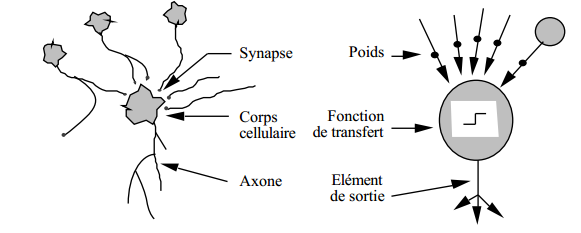
\includegraphics[scale=0.4]{images/chapter1/neurone_bio.png}\label{neurone}}
  \caption{Conception d'un neurone artificiel à partir d'un neurone biologique \\ Source : https://sites.google.com/site/tpeia9/home}
\end{center}
\end{figure}

\section{Un neurone}

\begin{definition}[Neurone]
Un neurone est modélisé par une fonction $f$ de $\mathbb{R}^n$ dans $\mathbb{R}$. Elle est déterminée par trois paramètres : un vecteur de poids $w \in \mathbb{R}^n$, un biais $b \in \mathbb{R}$ et une fonction d'activation $g$. La fonction $f$ se réécrit alors :

\begin{equation}
\forall x \in \mathbb{R}^n, y = f(x) = g(w^Tx+b) = g(\sum_{i=1}^{n}{w_ix_i}+b)
\label{sortie_neurone1}
\end{equation}
\end{definition}

\begin{remark}
Il est usuel de rajouter une composante $x_0$ égale à 1 à chaque entrée afin de pouvoir considérer le biais comme un simple poids. Avec cette convention, la formule \ref{sortie_neurone1} devient :

\begin{equation}
\forall x \in \mathbb{R}^n, y = f(x) = g(w^Tx) = g(\sum_{i=0}^{n}{w_ix_i})
\label{sortie_neurone2}
\end{equation}
\end{remark}

L'analogie avec le neurone biologique est ici claire. La fonction prend plusieurs entrées que l'on peut assimiler aux dendrites, les pondère et renvoie une sortie scalaire qui correspond à l'axone.

La figure \ref{neurone} montre une représentation graphique d'un neurone.

\begin{figure}
\begin{center}
\pagestyle{empty}
\begin{tikzpicture}[scale=0.6][line cap=round,line join=round,>=triangle 45,x=1.0cm,y=1.0cm]
\clip(-7.42,-11.35) rectangle (16.51,6.37);
\draw(0,2) circle (1cm);
\draw(0,-1) circle (1cm);
\draw(0,-4) circle (1cm);
\draw(0,-7) circle (1cm);
\draw(7,-2.5) circle (1cm);
\draw [->] (1,2) -- (6,-2.5);
\draw [->] (1,-1) -- (6,-2.5);
\draw [->] (1,-4) -- (6,-2.5);
\draw [->] (1,-7) -- (6,-2.5);
\draw [->] (8,-2.5) -- (10,-2.5);
\draw (8.5,-1.8) node[anchor=north west] {$ y $};
\draw (-1,2.4) node[anchor=north west] {$ x_0=1 $};
\draw (-0.45,-0.7) node[anchor=north west] {$ x_1 $};
\draw (-0.45,-3.7) node[anchor=north west] {$ x_2 $};
\draw (-0.45,-6.7) node[anchor=north west] {$ x_3 $};
\draw (3.3,0.5) node[anchor=north west] {$ w_0 $};
\draw (2.95,-0.9) node[anchor=north west] {$ w_1 $};
\draw (2.95,-2.3) node[anchor=north west] {$ w_2 $};
\draw (3.3,-3.5) node[anchor=north west] {$ w_3 $};
\draw (5.9,-1.9) node[anchor=north west] {$ g(w^Tx) $};
\end{tikzpicture}
\caption{Représentation graphique d'un neurone. Le biais est ici considéré comme le poids associé à une entrée constante égale à 1.}
\label{neurone}
\end{center}
\end{figure}

Les principales fonctions d'activation sont : 

\begin{itemize}
\item $Id : x \mapsto x$ dite identité;
\item $u : x \mapsto 1_{x \geq 0}$ dite échelon ou fonction de Heavyside ;
\item $\tanh : x \mapsto \tanh(x)$ dite tangente hyperbolique ;
\item $\sigma : x \mapsto \frac{1}{1+\exp(-x)}$ dite sigmoïde de part de sa forme en S;
\item $ReLU : x \mapsto max(0, x)$ dite ReLU (rectified linear unit).
\end{itemize}

La figure \ref{fonctions_activation} montre les graphes de ces différentes fonctions et permet de visualiser les différences entre celles-ci.

\begin{figure}
\begin{center}
\begin{tabular}{cc}
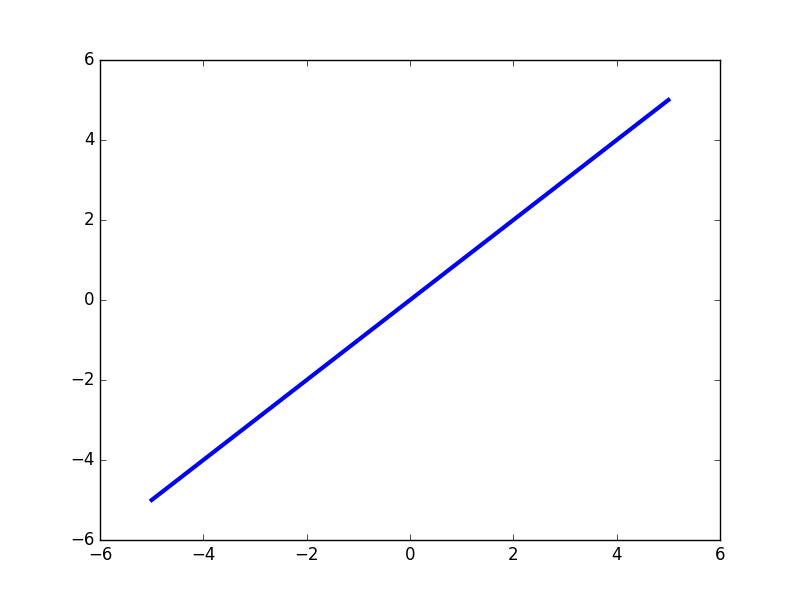
\includegraphics[scale=0.25]{images/chapter1/id.png} & 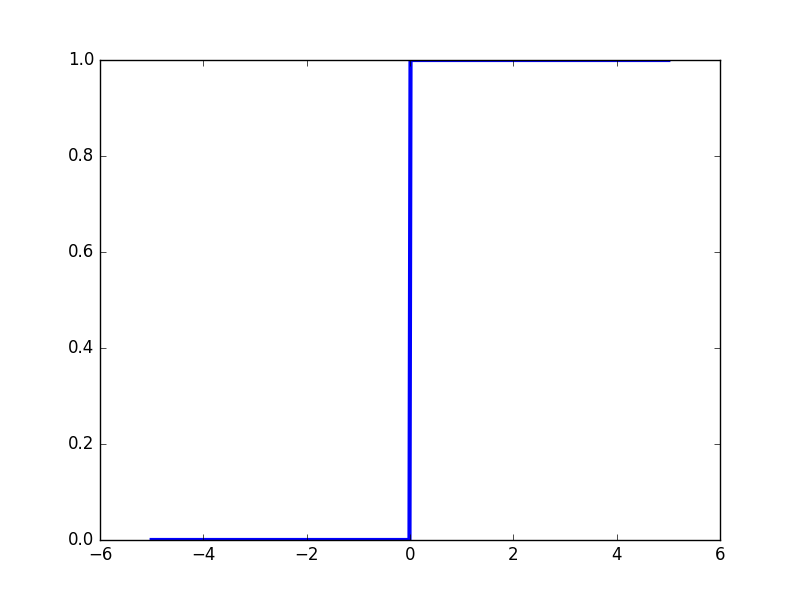
\includegraphics[scale=0.25]{images/chapter1/u.png} \\
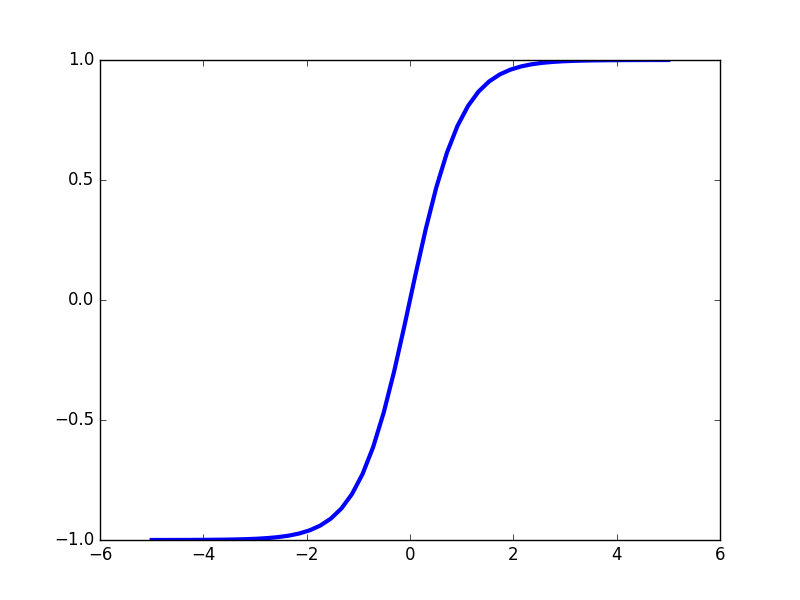
\includegraphics[scale=0.25]{images/chapter1/tanh.png} & 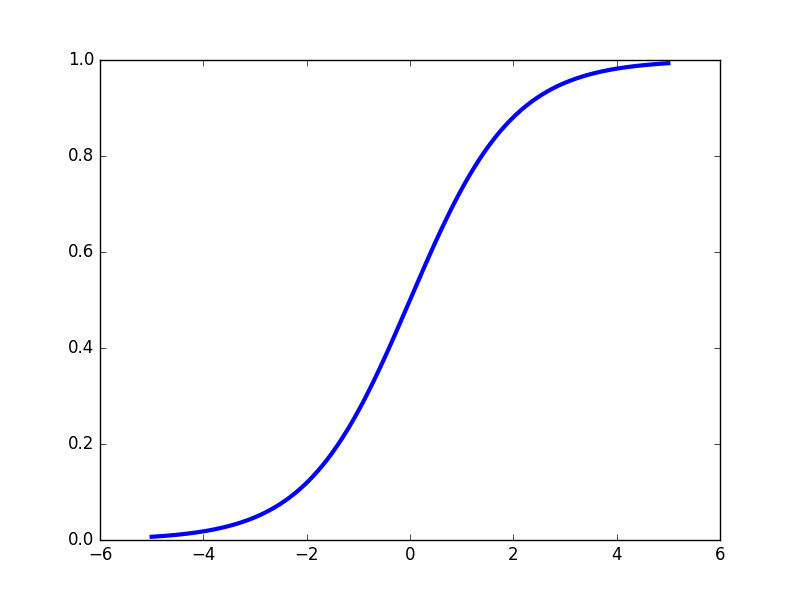
\includegraphics[scale=0.25]{images/chapter1/s.png} \\
\multicolumn{2}{c}{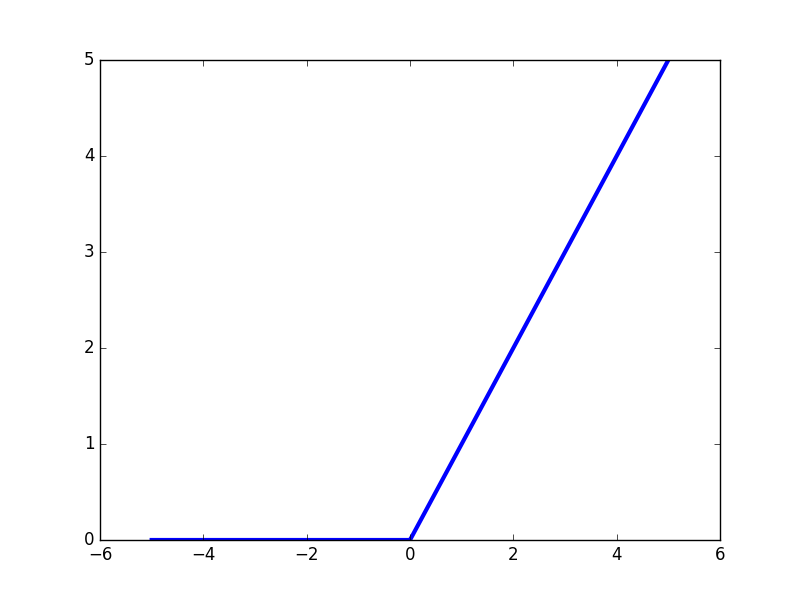
\includegraphics[scale=0.25]{images/chapter1/relu.png}}
\end{tabular}
\caption{Graphe entre -5 et 5 de la fonction identité (en haut à gauche), de l'échelon (en haut à droite), de la tangente hyperbolique (au milieu à gauche), de la sigmoïde (au milieu à droite) et de ReLU (en bas).} 
\label{fonctions_activation}
\end{center}
\end{figure}

Il est possible de se servir d'un neurone seul pour résoudre des problèmes de classification ou de régression. Détaillons quelques exemples importants.

\begin{example}[Perceptron]
Un neurone avec comme fonction d'activation un échelon sépare l'espace en deux demis espaces séparés par un hyperplan de vecteur normal $w$. En effet :

\begin{itemize}
\item $ \forall x \in \mathbb{R}^n, w^Tx < 0 \Rightarrow f(x) = 0$
\item $ \forall x \in \mathbb{R}^n w^Tx \geq 0 \Rightarrow f(x) = 1$
\end{itemize}

La figure \ref{hyperplan} illustre cette séparation. Ce cas particulier de neurone est couramment appelé perceptron.
\end{example}

\begin{figure}
\begin{center}
\pagestyle{empty}
\definecolor{qqqqff}{rgb}{0,0,1}
\definecolor{ffqqqq}{rgb}{1,0,0}
\begin{tikzpicture}[line cap=round,line join=round,>=triangle 45,x=1.0cm,y=1.0cm]
\draw[->,color=black] (-5.42,0) -- (5.45,0);
\foreach \x in {-5,-4,-3,-2,-1,1,2,3,4,5}
\draw[shift={(\x,0)},color=black] (0pt,2pt) -- (0pt,-2pt) node[below] {\footnotesize $\x$};
\draw[->,color=black] (0,-2.99) -- (0,5.07);
\foreach \y in {-2,-1,1,2,3,4,5}
\draw[shift={(0,\y)},color=black] (2pt,0pt) -- (-2pt,0pt) node[left] {\footnotesize $\y$};
\draw[color=black] (0pt,-10pt) node[right] {\footnotesize $0$};
\clip(-5.42,-2.99) rectangle (5.45,5.07);
\fill[line width=0pt,color=ffqqqq,fill=ffqqqq,fill opacity=0.1] (-12.7,-3.03) -- (15.5,5.76) -- (10.12,27.67) -- (-20,20) -- cycle;
\fill[line width=0pt,color=qqqqff,fill=qqqqff,fill opacity=0.1] (-12.7,-3.03) -- (-3.47,-28.78) -- (29.71,-17.95) -- (15.5,5.76) -- cycle;
\draw [domain=-5.42:5.45] plot(\x,{(-1.14-0.38*\x)/-1.22});
\draw [->] (1.12,1.28) -- (0.74,2.5);
\draw (0.74,2.89) node[anchor=north west] {$ w $};
\end{tikzpicture}
\caption{Hyperplan séparateur dans un espace à deux dimensions correspondant à un certain vecteur de poids $w$. La partie rouge correspond aux entrées classifiées 1 et en bleue celles qui sont classifiées 0.}
\label{hyperplan}
\end{center}
\end{figure}

\begin{example}[Régression logistique]
Si la fonction d'activation est une sigmoïde, la sortie du neurone peut être interprétée comme la probabilité $p(y=1|x)$. Par conséquent, le neurone classifie un exemple dans la classe 1 si la sortie est supérieure à $0.5$ et dans la classe 0 sinon. On parle ici de régression logistique. L'espace est toujours séparée en deux parties par un hyperplan, $H = \{x, f(x)=0.5\}$. Cependant maintenant les valeurs associées aux entrées sont continues entre $0$ et $1$. La figure \ref{regression_logistique} permet de visualiser cette différence. Dans la suite de ce document, des graphes de ce type seront utilisés à plusieurs reprises afin de pouvoir visualiser l'action d'un réseau de neurones.
\end{example}

\begin{figure}
\begin{center}
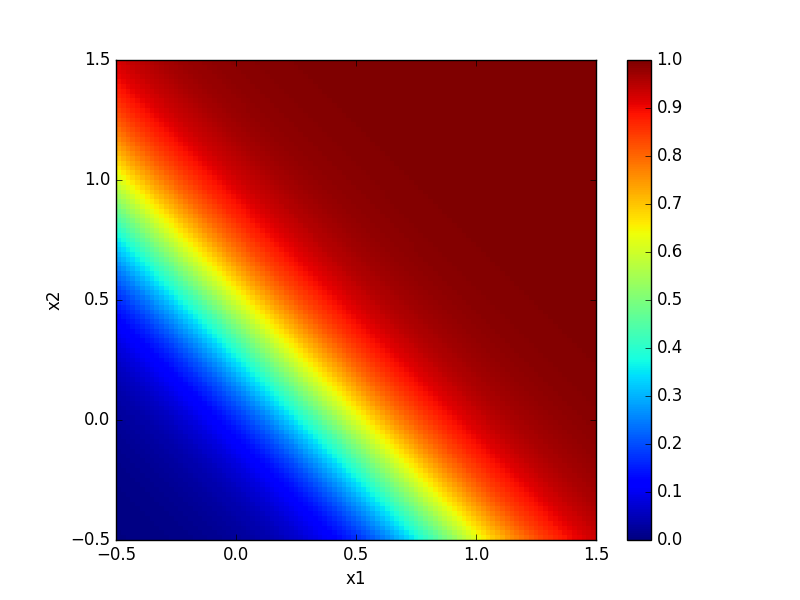
\includegraphics[scale=0.5]{images/chapter1/or.png}
\caption{Sortie d'une régression logistique prenant en entrée un vecteur de $\mathbb{R}^2$ sur $[-0.5, 1.5] \times [-0.5, 1.5]$. L'axe $x_1$ et l'axe $x_2$ correspondent respectivement à la première et à la deuxième coordonnée de l'entrée.}
\label{regression_logistique}
\end{center}
\end{figure}

\begin{example}[Régression linéaire]
Finalement, si la fonction d'activation est la fonction identité, le neurone sera capable d'atteindre toutes les valeurs réelles. Il pourra donc résoudre un problème de régression. Il s'agit de la régression linéaire.
\end{example}

Le point commun entre tous les neurones est qu'ils sont seulement capable de modéliser des interactions linéaires entre les entrées. Cependant, à partir d'un ensemble de données, il est possible d'utiliser des neurones pour modéliser des interactions non linéaires entre les différentes composantes des entrées. Pour cela, il faut transformer les entrées afin de créer de nouvelles composantes. Par exemple, prenons un ensemble de données tel que les points ont le label $1$ s'ils sont dans le disque de rayon 0.5 et de centre $(0;0)$ et $0$ sinon. Un exemple d'un tel ensemble de donnée est visible sur la figure \ref{disque}. En l'état, cet ensemble n'est pas linéairement séparable et donc un neurone simple ne peut pas le classifier correctement. Cependant si une transformation telle que $x \mapsto (x_1, x_2, x_1x_2, x_1^2, x_2^2)$ est appliquée aux exemples. Les points sont maintenant linéairement séparables dans ce nouvel espace. Il est alors possible d'utiliser un neurone afin de classifier correctement l'ensemble. Ces résultats sont présents sur la figure \ref{disque}.

\begin{figure}
\begin{center}
\begin{tabular}{cc}
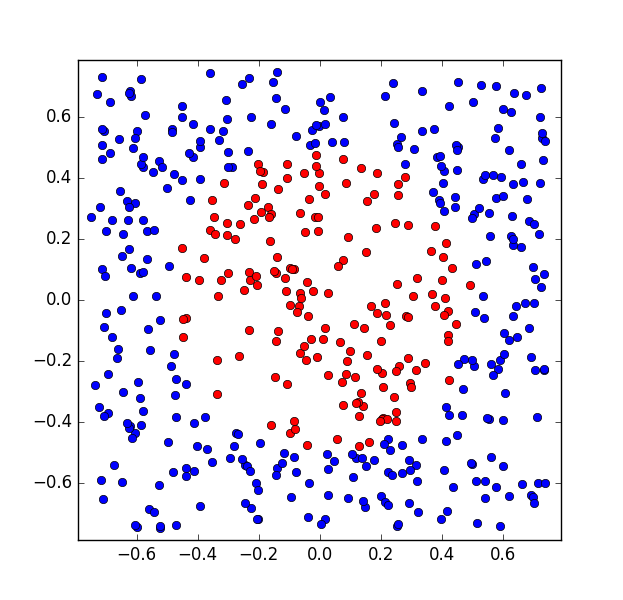
\includegraphics[scale=0.35]{images/chapter1/disk_dataset.png} & 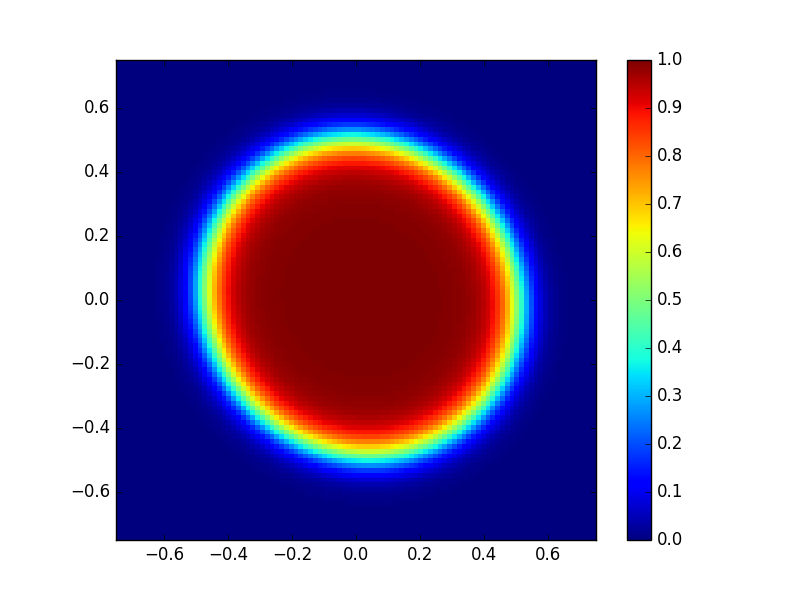
\includegraphics[scale=0.35]{images/chapter1/disk_learned.png} \\
\end{tabular}
\caption{À gauche un ensemble de données de 500 points. Les points à l'intérieur du cercle de rayon 0.5 et de centre $(0; 0)$ sont en rouge, les autres en bleu. À droite, la représentation du disque apprise par le neurone.} 
\label{disque}
\end{center}
\end{figure}

En conclusion, un neurone est une fonction relativement simple permettant de modéliser des interactions linéaires entre ses entrées. Dans la partie suivante, nous verrons comment associer ces neurones afin de créer des modèles plus complexes.

\section{Un réseau de neurones}

\begin{definition}[Réseau de neurones]
Un réseau de neurones est défini par un graphe orienté $\mathcal{G}(V, A)$ où les n\oe{}uds sont des neurones et les arêtes des liens entre les neurones et par un ensemble de neurones d'entrée $V_{in} \subset V$ et de neurones de sorties $V_{out} \subset V$. Une arête partant d'un neurone $i$ vers un neurone $j$ signifie que la sortie du neurone $i$ est une entrée pour le neurone $j$. Notons $f_{j}$ la fonction représentant le neurone $j$. Finalement, nous noterons un réseau $\mathcal{N}(V, A, V_{in}, V_{out}, f)$ où $f$ est l'ensemble des fonctions des neurones.
\end{definition}

Si nous notons $Pa$ l'application qui à un neurone renvoie les indices de ses parents et $Ch$ l'application qui à un neurone renvoie les indices de ses enfants. Alors la sortie du neurone $j$ est :

\begin{equation}
y_{j} = f_{j}((y_{i})_{i \in Pa(j)})
\label{eq_propagation}
\end{equation} 

Il existe certaines classes particulière de réseau de neurones. Tout d'abord, s'il contient des cycles, il sera dit récurrent. Dans le cas contraire, on parlera de réseau \textit{feedforward}. Puis s'il est possible de l'organiser sous forme de couches où les sorties des neurones d'une couche sont les entrées de la couche suivante, on parle de réseau de neurones multicouche dit aussi MLP (multilayer perceptron). Des exemples des différents types de réseaux sont présents sur la figure \ref{reseaux}.

\begin{figure}
\begin{center}
\begin{tabular}{cc}
\begin{tikzpicture}[scale=0.30][line cap=round,line join=round,>=triangle 45,x=1.0cm,y=1.0cm]
\clip(-3.5,-5.5) rectangle (13.5,7);
\draw(-1,4) circle (1cm);
\draw(-1,1) circle (1cm);
\draw(-1,-2) circle (1cm);
\draw(3,3) circle (1cm);
\draw(3,-1) circle (1cm);
\draw(7,3) circle (1cm);
\draw(11,3) circle (1cm);
\draw(11,-1) circle (1cm);
\draw [->] (0,4) -- (2,3);
\draw [->] (0,1) -- (2,3);
\draw [->] (0,-2) -- (2,-1);
\draw [->] (0,1) -- (2,-1);
\draw [->] (3,0) -- (3,2);
\draw(7,-1) circle (1cm);
\draw [->] (7,2) -- (4,-1);
\draw [->] (4,3) -- (6,3);
\draw [->] (4,-1) -- (6,-1);
\draw [->] (7,0) -- (7,2);
\draw [->] (8,3) -- (10,3);
\draw [->] (8,-1) -- (10,-1);
\draw [rotate around={90:(-1,1)},dash pattern=on 3pt off 3pt] (-1,1) ellipse (5.22cm and 1.5cm);
\draw (-3.5,-4.15) node[anchor=north west] {$ Entrées $};
\draw [rotate around={90:(11,1)},dash pattern=on 3pt off 3pt] (11,1) ellipse (4.25cm and 1.45cm);
\draw (8.8,-3.21) node[anchor=north west] {$ Sorties $};
\draw (-1.7,4.6) node[anchor=north west] {$ 1 $};
\draw (-1.95,1.6) node[anchor=north west] {$ x_1 $};
\draw (-1.95,-1.4) node[anchor=north west] {$ x_2 $};
\draw (2.1,3.9) node[anchor=north west] {$ f_1 $};
\draw (2.1,-0.1) node[anchor=north west] {$ f_2 $};
\draw (6,3.9) node[anchor=north west] {$ f_3 $};
\draw (6,-0.1) node[anchor=north west] {$ f_4 $};
\draw (10,3.7) node[anchor=north west] {$ y_1 $};
\draw (10,-0.3) node[anchor=north west] {$ y_2 $};
\end{tikzpicture} & \begin{tikzpicture}[scale=0.3][line cap=round,line join=round,>=triangle 45,x=1.0cm,y=1.0cm]
\clip(-3.94,-7.74) rectangle (13.14,4.91);
\draw(-1,2) circle (1cm);
\draw(-1,-1) circle (1cm);
\draw(-1,-4) circle (1cm);
\draw(3,1) circle (1cm);
\draw(3,-3) circle (1cm);
\draw(7,-1) circle (1cm);
\draw(11,-1) circle (1cm);
\draw [->] (0,2) -- (2,1);
\draw [->] (0,-1) -- (2,1);
\draw [->] (0,-4) -- (2,-3);
\draw [->] (4,1) -- (6,-1);
\draw [->] (3,-2) -- (3,0);
\draw [->] (6,-1) -- (4,-3);
\draw [->] (8,-1) -- (10,-1);
\draw [rotate around={0:(4.5,-1)},dash pattern=on 3pt off 3pt] (4.5,-1) ellipse (3.81cm and 3.5cm);
\draw (2.7,-4.43) node[anchor=north west] {$ Cycle $};
\end{tikzpicture} \\
\begin{tikzpicture}[scale=0.3][line cap=round,line join=round,>=triangle 45,x=1.0cm,y=1.0cm]
\clip(-3.8,-5.74) rectangle (12.92,6.64);
\draw(-1,1) circle (1cm);
\draw(-1,4) circle (1cm);
\draw(-1,-2) circle (1cm);
\draw(3,4) circle (1cm);
\draw(3,-2) circle (1cm);
\draw(3,1) circle (1cm);
\draw(7,1) circle (1cm);
\draw(10,4) circle (1cm);
\draw(10,-2) circle (1cm);
\draw [->] (0,4) -- (2,4);
\draw [->] (0,1) -- (2,4);
\draw [->] (0,1) -- (2,-2);
\draw [->] (0,-2) -- (2,-2);
\draw [->] (3,-1) -- (3,0);
\draw [->] (3,3) -- (3,2);
\draw [->] (4,1) -- (6,1);
\draw [->] (4,-2) -- (6,1);
\draw [->] (4,4) -- (6,1);
\draw [->] (8,1) -- (9,4);
\draw [->] (8,1) -- (9,-2);
\draw [->] (4,-2) -- (9,-2);
\draw [->] (4,4) -- (9,4);
\end{tikzpicture} & \begin{tikzpicture}[scale=0.24][line cap=round,line join=round,>=triangle 45,x=1.0cm,y=1.0cm]
\clip(-8.76,-5.24) rectangle (13.65,11.36);
\draw(-2,6) circle (1cm);
\draw(-2,3) circle (1cm);
\draw(-2,0) circle (1cm);
\draw(2,3) circle (1cm);
\draw(2,6) circle (1cm);
\draw(2,0) circle (1cm);
\draw(2,-3) circle (1cm);
\draw(2,9) circle (1cm);
\draw(6,6) circle (1cm);
\draw(6,3) circle (1cm);
\draw(6,0) circle (1cm);
\draw(10,3) circle (1cm);
\draw [->] (-1,6) -- (1,9);
\draw [->] (-1,6) -- (1,6);
\draw [->] (-1,6) -- (1,3);
\draw [->] (-1,6) -- (1,0);
\draw [->] (-1,3) -- (1,9);
\draw [->] (-1,3) -- (1,6);
\draw [->] (-1,3) -- (1,3);
\draw [->] (-1,3) -- (1,0);
\draw [->] (-1,0) -- (1,0);
\draw [->] (-1,0) -- (1,3);
\draw [->] (-1,0) -- (1,6);
\draw [->] (-1,0) -- (1,9);
\draw [->] (3,9) -- (5,6);
\draw [->] (3,6) -- (5,6);
\draw [->] (3,3) -- (5,6);
\draw [->] (3,0) -- (5,6);
\draw [->] (3,6) -- (5,3);
\draw [->] (3,3) -- (5,3);
\draw [->] (3,3) -- (5,0);
\draw [->] (3,9) -- (5,3);
\draw [->] (3,9) -- (5,0);
\draw [->] (3,6) -- (5,0);
\draw [->] (3,0) -- (5,0);
\draw [->] (3,0) -- (5,3);
\draw [->] (-1,6) -- (1,-3);
\draw [->] (-1,3) -- (1,-3);
\draw [->] (-1,0) -- (1,-3);
\draw [->] (3,-3) -- (5,0);
\draw [->] (3,-3) -- (5,3);
\draw [->] (3,-3) -- (5,6);
\draw [->] (7,6) -- (9,3);
\draw [->] (7,3) -- (9,3);
\draw [->] (7,0) -- (9,3);
\end{tikzpicture} \\
\end{tabular}
\caption{Exemples de réseaux de neurones. Un réseau de neurones quelconque (en haut à gauche),  récurrent (en haut à droite), feedforward (en bas à gauche) et multicouche (en bas à droite).} 
\label{reseaux}
\end{center}
\end{figure}

Dans les sections suivantes, seront étudiés les algorithmes pour évaluer un réseau de neurones puis pour l’entraîner. Cependant, seulement les algorithmes dans le cadre d'un réseau de neurones feedforward seront abordés. Les algorithmes concernant les réseaux de neurones récurrent seront abordés dans la partie \autoref{chap:Réseaux de neurones récurrents}.

\section{Propagation}

L'algorithme de propagation dans le cadre des réseaux feedforward est très simple. Il suffit de mettre à jour les neurones d'entrée puis d'appliquer la formule \ref{eq_propagation} récursivement en partant des neurones dans $V_{out}$.

Ainsi, un premier algorithme naïf est :

\begin{algorithm} 
\begin{algorithmic}
\Procedure{$evaluer\_reseau$}{$\mathcal{N}(V, A, V_{in}, V_{out}, f), x$}
\Function{$evaluer\_neurone$}{$j$}
	\If{$j \in V_{in}$}
    	\State \Return $x_j$
	\Else
		\State $t \leftarrow (evaluer\_neurone(i), i \in Pa(j))$
		\State \Return $f_j(t)$
	\EndIf
\EndFunction

\For{$j \in V_{out}$}
	\State $y_j \leftarrow evaluer\_neurone(j)$ 
\EndFor
\EndProcedure
\end{algorithmic} 
\caption{Algorithme naïf d'évaluation d'un réseau de neurone feedforward. Il prend en entrée un réseau de neurone et un vecteur d'entrée pour le réseau de neurone.}
\end{algorithm}

Cette version n'est pas du tout efficace, elle calcule plusieurs fois la sortie de chaque neurone. Si le graphe est densément connecté, l'algorithme aura un coût temporel extrêmement élevé. Une amélioration simple consiste à rajouter de la mémoïsation afin de garantir que la sortie de chaque neurone sera calculée au plus une fois. Le pseudo-code de cet algorithme correspond à l'algorithme \ref{propagation_memoisation}.

\begin{algorithm} 
\begin{algorithmic}
\Procedure{$evaluer\_reseau$}{$\mathcal{N}(V, A, V_{in}, V_{out}, f), x$}
\Function{$evaluer\_neurone$}{$j$}
	\If{$déjàCalculé[j]$ est $faux$}
		\State $t \leftarrow (evaluer\_neurone(i), i \in Pa(j))$
		\State $y_j \leftarrow f_j(t)$
		\State $déjàCalculé[j] \leftarrow vrai$
	\EndIf
	\State \Return $y_j$
\EndFunction

\State Initialiser un tableau $dejaCalculé$ de longueur $|V|$ à $faux$.
\For{$i \in V_{in}$}
	\State $y_i \leftarrow x_i$
	\State $déjàCalculé[i] \leftarrow vrai$ 
\EndFor
\For{$j \in V_{out}$}
	\State $evaluer\_neurone(j)$ 
\EndFor
\EndProcedure
\end{algorithmic}
\caption{Algorithme d'évaluation d'un réseau de neurone feedforward utilisant la mémoïsation afin de ne pas recalculer plusieurs fois la sortie d'un neurone.}
\label{propagation_memoisation}
\end{algorithm}

Cet algorithme calcule au plus une fois la sortie de chaque neurone et il appelle $evaluer\_neurone$ au plus $|A|$ fois, il a donc un coût temporel en $O(|V|+|A|)$. Ce qui est a priori le coût optimal.

\section{Fonctions de coût}

Avant de parler des algorithmes d'apprentissage et de la manière de modifier les poids avant d'approcher une fonction, nous allons revenir sur les fonctions de coût. Dans la suite, nous justifierons l'utilisation et le bien-fondé des fonctions de coût les plus courantes.

Il sera détaillé trois fonctions de coût : une pour la régression, une pour la classification binaire et une pour la classification à plusieurs classes. La même méthode sera utilisée à chaque fois : un modèle sera proposé puis la fonction de coût sera déduite en utilisant le principe du maximum de vraisemblance.

\begin{definition}[Fonction de vraisemblance]
Si $x_1, ..., x_n$ sont des échantillons générés indépendamment par une probabilité $p_{\theta}$ la vraisemblance de l'échantillon est alors :
$$
L(\theta) = \prod_{i=1}^{N}{p_{\theta}(x^{(i)})}
$$
\end{definition}

\begin{remark}
Dans notre cas, les échantillons $(x_1, y_1), ..., (x_n, y_n)$ sont générés par la loi $p_{\theta}(y|x)$ où $\theta$ sont les paramètres du modèle, la vraisemblance est donc :
$$
L(\theta) = \prod_{i=1}^{N}{p_{\theta}(y^{(i)}|x^{(i)})}
$$
\end{remark}

\begin{definition}[Maximum de vraisemblance]
Le paramètre $\theta$ maximise la vraisemblance si $\theta \in argmax L(\theta')$.
\end{definition}

\begin{remark}
Maximiser la vraisemblance revient donc à rechercher le maximum d'une fonction.
\end{remark}

\begin{remark}
Au lieu de maximiser la vraisemblance, nous allons minimiser l'opposé du logarithme de la vraisemblance (\textit{negative log-likelihood} en anglais). On obtient alors :
\begin{equation}
NLL(\theta) = -\sum_{i=1}^{N}{\log{p_{\theta}(y^{(i)}|x^{(i)})}}
\label{NLL}
\end{equation}
Cette forme est préférée car la somme est plus facile à dériver que le produit. En outre, l'opposé du logarithme de la vraisemblance est pris pour se ramener à un problème de minimisation.
\end{remark}

\subsection{Régression}

Dans un problème de régression, il est courant de choisir comme modèle :

\begin{equation}
p_{\theta}(y|x) \sim \mathcal{N}(\hat{y}(x, \theta), \sigma) \Leftrightarrow p_{\theta}(y|x) = \frac{1}{\sqrt{2\pi}\sigma}\exp{(\frac{-(y - \hat{y})^2}{2\sigma^2})}
\label{modele_normale}
\end{equation}

Où $\theta$ est l'ensemble des poids de notre réseau, $\hat{y}(x, \theta)$ est la sortie de notre réseau quand l'entrée est $x$ et $\sigma$ une constante positive. On se permettra de noter seulement $\hat{y}(x)$ au lieu de $\hat{y}(x, \theta)$ pour plus de légèreté.


En remplaçant $p_{\theta}$ par l'expression \ref{modele_normale} dans l'équation \ref{NLL}, on obtient :

\begin{equation}
NLL(\theta) = \sum_{i=1}^{N}{(y^{(i)} - \hat{y}(x^{(i)}))^2} + C
\end{equation}

où $C$ est une constante.

Dans le problème de minimisation, la constante peut être négligée et il est possible de multiplier par une constante positive sans changer le problème. On déduit que sous cette modélisation, une fonction de coût obtenue par le principe de maximum de vraisemblance est :

\begin{equation}
E = \frac{1}{N}\sum_{i=1}^{N}{(y^{(i)} - \hat{y}(x^{(i)}))^2} = \frac{1}{N}\sum_{i=1}^{N}{e(y^{(i)}, \hat{y}(x^{(i)}))}
\end{equation}

avec $e : (x, y) \mapsto (x - y)^2$. Cette fonction est appelée erreur quadratique moyenne (\textit{mean squared error} en anglais).

\subsection{Classification binaire}

Dans le cas de la classification binaire, à $x$ fixé, $p(y|x)$ suit une loi de Bernoulli. Un modèle possible est donc :

\begin{equation}
p_{\theta}(y|x) \sim \mathcal{B}(\hat{y}(x, \theta)) \Leftrightarrow p_{\theta}(y|x) = 
\left\{
    \begin{array}{ll}
        \hat{y}(x) \text{ si } y = 1 \\
        1 - \hat{y}(x) \text{ sinon}
    \end{array}
\right.
\label{modele_bernoulli}
\end{equation}

La formule \ref{modele_bernoulli} peut se réécrire de manière plus compacte :
\begin{equation}
p_{\theta}(y|x) = \hat{y}(x)^y(1-\hat{y}(x))^{1-y}
\label{modele_bernoulli_compact}
\end{equation}

En utilisant cette dernière forme, on obtient que l'expression de la \textit{negative log-likelihood} est : 

\begin{equation}
NLL(\theta) = -\sum_{i=1}^{N}{y^{(i)}\log\hat{y}(x^{(i)})+(1-y^{(i)})\log(1-\hat{y}(x^{(i)}))}
\end{equation}

On en déduit de même que précédemment que notre fonction de coût est :

\begin{equation}
E = \frac{1}{N}\sum_{i=1}^{N}{-(y^{(i)}\log\hat{y}(x^{(i)})+(1-y^{(i)})\log(1-\hat{y}(x^{(i)})))} = \frac{1}{N}\sum_{i=1}^{N}{e(y^{(i)}, \hat{y}(x^{(i)}))}
\end{equation}

avec $e : (x, y) \mapsto -(x \log y + (1-x)\log(1-y))$.

\subsection{Classification à plusieurs classes}

Finalement, dans le cas d'une classification à plusieurs classes, $p(y|x)$ est une loi Multinoulli à $x$ fixé. Si la sortie $\hat{y}$ du réseau est un vecteur de longueur $M$ avec $M$ le nombre de classes, une sortie possible est :

\begin{equation}
p_{\theta}(y|x) \sim \mathcal{M}(\hat{y}(x, \theta)_0, ..., \hat{y}(x, \theta)_{M-1}) \Leftrightarrow p_{\theta}(y|x) = \hat{y}(x)_y
\label{modele_multinoulli}
\end{equation}

La \textit{negative log-likelihood} associée est donc :

\begin{equation}
NLL(\theta) = -\sum_{i=1}^{N}{\log \hat{y}(x^{(i)})_{y^{(i)}}}
\label{NLL_multinoulli}
\end{equation}

Posons pour tout $i \in \{0, ..., M-1\}$, $\tau^{(i)} \in \mathbb{R}^M$ le vecteur tel que :

$$ \tau^{(i)}_j = 
\left\{
    \begin{array}{ll}
        1 \text{ si } i = j \\
        0 \text{ sinon}
    \end{array}
\right.
$$

Il est alors possible de réécrire la formule \ref{NLL_multinoulli} en utilisant ces vecteurs :

\begin{equation}
NLL(\theta) = \sum_{i=1}^{N}{-\sum_{j=0}^{M-1}{\tau^{(y^{(i)})}_j\log \hat{y}(x^{(i)})_j}}
\end{equation}

Enfin en introduisant l'entropie croisée $H$ définie de manière générale par :

$$
H(p, q) = -\sum_{x}{p(x)\log q(x)}
$$

On obtient que :

\begin{equation}
NLL(\theta) = \sum_{i=1}^{N}{H(\tau^{(y^{(i)})}, \hat{y}(x^{(i)}))}
\end{equation}

On a remplacé $y$ par un vecteur prenant un $1$ à la position $y$, une telle transformation est couramment appelé encodage \textit{one-hot}. 

Notre fonction de coût sera donc :

\begin{equation}
E = \frac{1}{N}\sum_{i=1}^{N}{H(\tau^{(y^{(i)})}, \hat{y}(x^{(i)}))} = \frac{1}{N}\sum_{i=1}^{N}{e(y^{(i)}, \hat{y}(x^{(i)}))}
\end{equation}

Avec $e : (x, y) \mapsto H(\tau^x, y)$. Cette fonction de coût est naturellement appelée entropie croisée (\textit{cross-entropy} en anglais).

\section{Descente du gradient}

Étant donné une fonction de coût $E$, l'objectif de l'apprentissage est de déterminer les poids permettant de minimiser $E$. Dans l'idéal, il faudrait pouvoir exprimer $E$ en fonction des poids, dériver $E$ par rapport à chaque poids puis chercher les valeurs des poids atteignant les minimas. Malheureusement, dans la plupart des cas, il est impossible d'avoir de telles solutions analytiques.

Une réponse à ce problème est la descente du gradient. Le principe est simple, il s'agit d'un procédé itératif consistant à modifier légèrement les valeurs des poids afin qu'à chaque étape $E$ décroisse.  En notant, $\theta$ le vecteur contenant les poids de tous les neurones du réseau. La valeur de ces poids changera à chaque itération, par conséquent, notons $\theta(t)$ la valeur de $\theta$ à l'itération $t$. La direction selon laquelle $E$ augmente le plus est $\frac{\partial E}{\partial \theta}$, la direction selon laquelle $E$ décroît le plus est donc $-\frac{\partial E}{\partial \theta}$. Si les poids sont modifiés en se déplaçant dans cette direction d'un pas $\eta(t)$ assez petit, le coût diminuera. L'équation d'évolution est donnée par \ref{mise_a_jour_poids}.

\begin{equation}
\theta(t+1) = \theta(t) - \eta(t) \frac{\partial E}{\partial \theta}
\label{mise_a_jour_poids}
\end{equation}

Il existe plusieurs stratégies afin de choisir le pas $\eta(t)$. Dans un premier temps et pour plus de simplicité, nous choisirons un pas $\eta(t)=\eta$ constant.

\section{Rétropropagation du gradient}

L'application de l'algorithme précédant nécessite le calcul des dérivées partielles par rapport à chacun des poids du réseau de neurones. Prenons le neurone $j$ du réseau de neurone. Son entrée est notée $x_j$, sa sortie $y_j$, sa fonction d'activation $g_j$ et ses poids $w_j$. De plus, définissons la quantité intermédiaire $s_j = w_j^Tx_j$. La formule \ref{sortie_neurone2} appliquée à ce neurone est donc $y_j = g_j(w_j^Tx_j) = g(s_j)$. En utilisant la règle de la chaîne, on obtient que :

\begin{equation}
\frac{\partial E}{\partial w_j} = \frac{\partial E}{\partial y_j}\frac{\partial y_j}{\partial s_j}\frac{\partial s_j}{\partial w_j}
\label{dEdw_avant}
\end{equation}

On peut remarquer que le terme $\frac{\partial s_j}{\partial w_j}$ est égal à $x_j$ et que $\frac{\partial y_j}{\partial s_j} = g'(s_j)$ d'où l'égalité \ref{dEdw_avant} devient :

\begin{equation}
\frac{\partial E}{\partial w_j} = \frac{\partial E}{\partial y_j} g_j'(s_j) x_j
\label{dEdw}
\end{equation}

Afin de calculer $\frac{\partial E}{\partial y_j}$, utilisons le fait que la sortie du neurone $j$ est une des entrées de ses enfants. En notant $x_{i, j}$ l'entrée du neurone i correspondant à la sortie du neurone $j$, on a :

\begin{equation}
\frac{\partial E}{\partial y_j} = \sum_{i \in Ch(j)}{\frac{\partial E}{\partial x_{i,j}}}
\label{formule_retropropagation}
\end{equation}

La formule \ref{formule_retropropagation} montre que si on calcule $\frac{\partial E}{\partial x_i}$, la dérivée du coût par rapport aux entrées d'un neurone, il est aisé de calculer la dérivée du coût par rapport aux poids pour les parents de ce neurone. Or la dérivée du coût par rapport aux entrées d'un neurone est facilement calculable en utilisant l'égalité suivante :

\begin{equation}
\frac{\partial E}{\partial x_j} = \frac{\partial E}{\partial y_j}\frac{\partial y_j}{\partial s_j}\frac{\partial s_j}{\partial x_j} =  \frac{\partial E}{\partial y_j} g_j'(s_j) w_j
\label{dEdx}
\end{equation}

Finalement, en utilisant les formules \ref{dEdw}, \ref{formule_retropropagation} et \ref{dEdx}, il est possible de rétropropager le gradient et de calculer $\frac{\partial E}{\partial w_j}$ pour tout neurone $j$. On en déduit l'algorithme suivant :

\begin{algorithm} 
\begin{algorithmic}
\Procedure{$retropropager\_gradient$}{$\mathcal{N}(V, A, V_{in}, V_{out}, f), x, y$}
\Function{$calculer\_gradient$}{$j$}
	\If{$déjàCalculé_j$ est $faux$}
		\State $\frac{\partial E}{\partial y_j} \leftarrow \sum_{i \in Ch(j)}{calculer\_gradient(i)_j}$
		\State $\frac{\partial E}{\partial x_j} \leftarrow \frac{\partial E}{\partial y_j} g_j'(s_j) w_j$
		\State $\frac{\partial E}{\partial w_j} \leftarrow \frac{\partial E}{\partial y_j} g_j'(s_j) x_j$
		\State $déjàCalculé_j \leftarrow vrai$
	\EndIf
	\State \Return $\frac{\partial E}{\partial x_j}$
\EndFunction

\State Appeler $evaluer\_reseau(\mathcal{N}(V, A, V_{in}, V_{out}, f), x)$ et récupérer les entrées et sorties de chaque neurone
\State Initialiser un tableau $dejaCalculé$ de longueur $|V|$ à $faux$.
\For{$i \in V_{out}$}
	\State Calculer $\frac{\partial E}{\partial y_i}$
	\State $déjàCalculé_i \leftarrow vrai$ 
\EndFor
\For{$i \in V$}
	\State $calculer\_gradient(i)$ 
\EndFor
\EndProcedure
\end{algorithmic} 
\caption{Algorithme de rétropropagation du gradient dans un réseau de neurone feedforward.}
\label{propagation_memoisation2}
\end{algorithm}

Cet algorithme utilise la mémoïsation afin de ne pas calculer plusieurs fois les dérivées pour un neurone. On peut remarquer que cet algorithme est très similaire à celui de la propagation. Pour des raisons similaires, le coût temporel de la rétropropagation est aussi en $O(|V|+|A|)$.

\chapter{Une première implémentation}

\section{Motivation}

La première implantation a été faite sous Python avec pour but principal de rester le plus proche possible de l'architecture neuronale du réseau afin de pouvoir bien étudier le fonctionnement de l'algorithme d'apprentissage. Quitte à perdre en rapidité de calcul, nous avons ainsi décidé de créer des éléments neurones et un réseau composé de plusieurs de ces neurones. Cette approche permet une bonne compréhension des concepts de base des réseaux de neurones. Nous avons alors pu appliquer cette implémentation sur des cas simples (XOR notamment, cf Résultats), mais aussi obtenir un aperçu des optimisations possibles afin d'accélérer les calculs. Cela s'est effectivement rapidement révélé nécessaire.  

\section{Diagramme UML}

Suivant cette volonté de créer une première implémentation simple et intuitive, le diagramme UML comporte ainsi deux classes principales : une classe Neuron et une classe Network. Ainsi un réseau (network) sera composé de plusieurs neurones (neurons).

Le neurone a été défini comme une entité autonome, qui comporte des entrées et une sortie et est caractérisé par des poids ainsi que ses relations avec d'autres neurones (parents ou enfants). Il peut alors calculer la sortie si les sorties de ses parents ont préalablement été évaluées. Pour déterminer le gradient au niveau de chaque poids, il a tout d'abord besoin de ceux de ses enfants.


\begin{figure}
\begin{center}
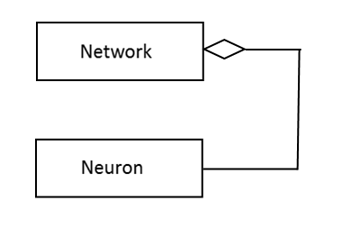
\includegraphics[scale=0.5]{images/uml_simplifie_imp1.png}
\caption{UML simplifié (à changer)}
\label{UML simplifié}
\end{center}
\end{figure}

\begin{figure}
\begin{center}
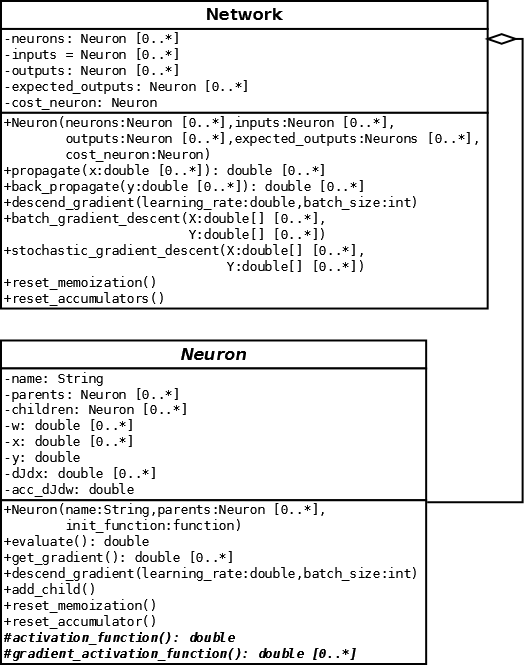
\includegraphics[scale=0.3]{images/uml_simplifie_maispastrop_imp1.png}
\caption{UML simplifié maispastrop}
\label{UML simplifié maispastrop}
\end{center}
\end{figure}

On répartit les neurones en différentes catégories selon leurs fonctions d'activation (sigmoïde, tangente hyperbolique, Softmax ou ReLu par exemple).

Ainsi la classe Neuron possède de nombreuses sous-classes correspondant à ces fonctions. En outre, il existe plusieurs sous-classes destinées aux neurones ayant un comportement particulier. On distingue ainsi BiasNeuron, qui permet d'ajouter un biais au niveau des entrées d'un autre neurone, InputNeuron correspondant simplement aux neurones d'entrées. L'ajout d'un neurone de coût (cost neuron) à la fin du réseau permet de calculer directement l'erreur lors de la propagation d'une entrée. Il faudra ainsi spécifier pour chaque input d'entrée la sortie attendue pour calculer le coût (avec un InputNeuron).

\begin{figure}
\begin{center}
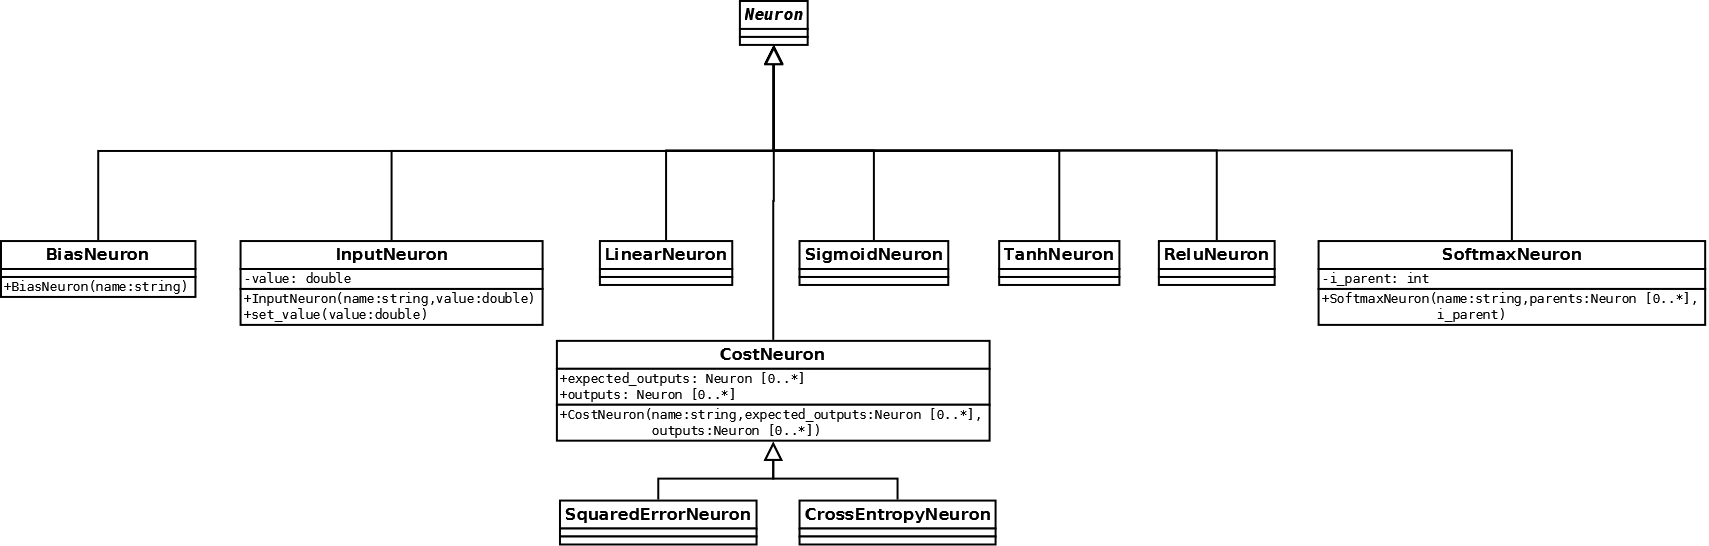
\includegraphics[scale=0.2]{images/uml_neurone_imp1.png}
\caption{Déclinaison de la classe neurone}
\label{uml_neurone_imp1}
\end{center}
\end{figure}


Les liens entre neurones ne seront pas mémorisées par le réseau. Cette tâche sera réalisée par les neurones eux-mêmes. Ainsi, chacun possédera en attribut une liste de parents et une liste d'enfants, ce qui lui permettra de se situer dans le réseau. Ces deux listes sont indispensables afin de propager le résultat de sortie du neurone et afin de rétropropager le gradient lors de l'algorithme d'apprentissage.
	
\section{Principe de fonctionnement}
Pour utiliser le programme, il suffit de créer le réseau de neurones voulu. On crée pour cela différents neurones (InputNeuron, SigmoidNeuron, CrossEntropyNeuron, ...) en spécifiant les parents à chaque fois. Le programme mettra lui même à jour les listes de parents et d'enfants de chaque neurone afin de créer les différentes relations entre neurones. On crée finalement le réseau (Network) en spécifiant les entrées, sorties, le neurone de coût et les neurones intermédiaires.
On peut alors appliquer deux fonctions principales sur le réseau. "Propagate" permet de calculer la sortie du réseau pour une entrée fournie en paramètre. "Batch\_propagation\_descent" permet d'appliquer l'algorithme de d'apprentissage basée sur la backpropagation du gradient pour un ensemble d'entrées, de sorties attendues et un learning rate $\eta$ donnés. 
Pour réaliser cet algorithme d'apprentissage, le programme sélectionne une entrée x et une sortie attendue y\_expected. Il applique ensuite un "propagate" afin d'obtenir la sortie y et le coût correspondant. Un backpropagate permet alors de faire remonter le gradient jusqu'à chaque neurone où il sera accumulé dans une variable acc\_dJdw. On réitère ce processus pour tous les couples x et y\_expected. Enfin, on met à jour les poids grâce à un "descent\_gradient" à l'aide de l'équation \ref{mise_a_jour_poids_batch} (valable pour un batch) :

\begin{equation}
w(t+1) = w(t) - \frac{\eta}{batch\_size}acc\_dJdw
\label{mise_a_jour_poids_batch}
\end{equation}

Nous avons utilisé diverses astuces afin d'améliorer l'efficacité de notre programme. Par exemple, la sigmoide est une fonction d'activation souvent utilisée. Elle est définie par $f(x) = \frac{1}{1+\exp(-x)}$. Au lieu d'entrée directement la formule complète de la dérivée, nous la simplifions en l'écrivant sous la forme $f'(x) = f(x) * (1 - f(x))$.
Nous utilisons deux variables acc\_dJdw et dJdx dans chaque neurone. La première permet d'accumuler les corrections à apporter aux poids que l'on applique à la fin du batch. dJdx sert de mémoization afin d'optimiser les calculs et de ne pas en faire d'inutiles. En effet, pour calculer son gradient, chaque neurone a besoin des gradients de ses enfants. Si nous ne mémorisions pas le gradient de chaque neurone dans dJdx, nous devrions le recalculer à chaque fois qu'un des parents le demande. Cela alourdirait énormément les calculs et ferait augmenter significativement le temps d'exécution. Ces deux variables doivent évidemment être réinitialisées à la fin du passage du batch de données.

\section{Résultats}

Afin de tester le fonctionnement de cette première application, nous avons commencé par le faire fonctionner sur un modèle simple: le XOR. Le but était donc de réaliser un réseau neuronal à deux entrées et une sortie qui fonctionne comme un XOR : il renvoie zéros si les entrées sont semblables (égales à un ou à zéro) et il renvoie un si elles sont différentes (l'une égale à un et l'autre à zéro). On entraine alors le réseau par le batch définition du XOR : les quatre couples (0;0), (0;1), (1;0) et (1;1). Le gradient est alors calculé en moyennant les résultats du réseau sur ces quatre entrées.
Cela a permis d'étudier et d'assurer le bon fonctionnement de l'implémentation.

Des premiers tests ont été réalisés avec un réseau avec une couche cachée de deux neurones. Les résultats sont alors plutôt mauvais : alors que théoriquement le XOR est réalisable avec cette architecture, nous avons pu observer que lors de l'exécution de l'algorithme, la descente du gradient a tendance à se bloquer dans un minimum local de la fonction de coût. 

\begin{figure}[!h]
\begin{center}
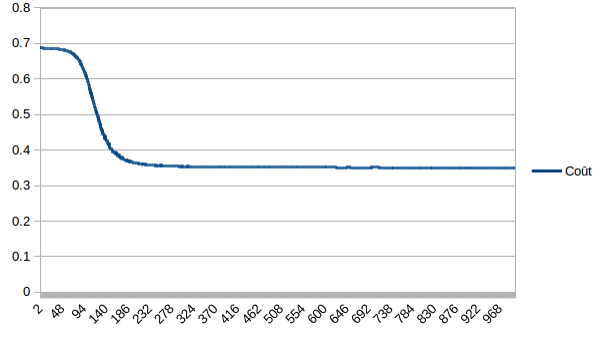
\includegraphics[scale=0.6]{images/xor_cost_function.png}
\caption{fonction de coût bloquée dans un minimum local}
\label{xor_cout_bloque}
\end{center}
\end{figure}

Nous avons alors pu remarquer que même en modifiant différents paramètres, (valeurs initiales des poids, learning rate ou les fonctions d'activation), cela restait inefficace, et les résultats obtenus ne correspondaient pas à la fonction xor que l'on attendait (voir figure \ref{xor_non_fonctionnel}).

\begin{figure}[!h]
\begin{center}
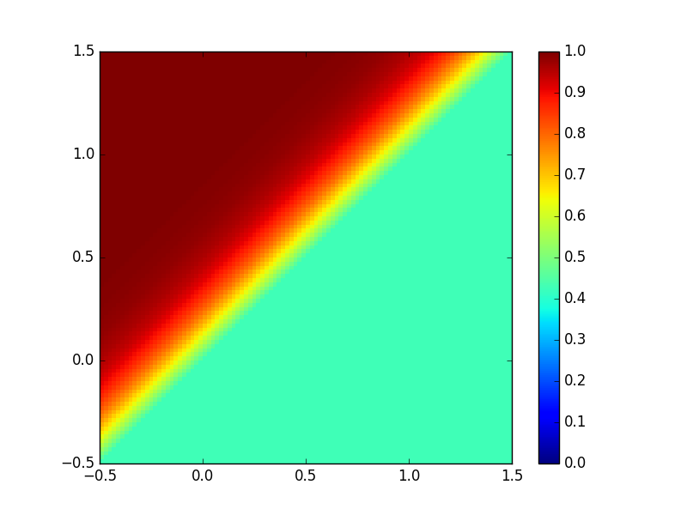
\includegraphics[scale=0.6]{images/xor_non_fonctionnel.png}
\caption{XOR bloqué dans un minimum local}
\label{xor_non_fonctionnel}
\end{center}
\end{figure}

Nous sommes alors passés sur une seconde architecture avec cette fois quatre neurones dans la couche intermédiaire cachée. On obtient cette fois de très bons résultats comme celui de la figure \ref{xor_relu_2_4}.

\begin{figure}[!h]
\begin{center}
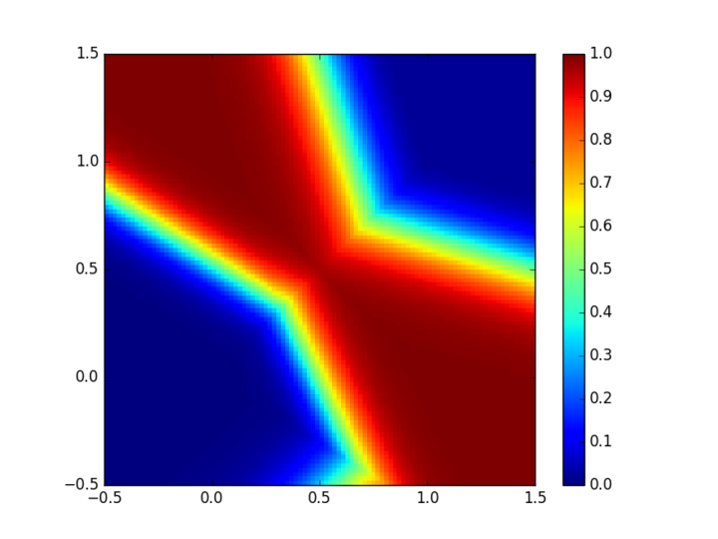
\includegraphics[scale=0.6]{images/xor_relu_2_4.png}
\caption{2 couches cachées de 4 neurones-ReLu}
\label{xor_relu_2_4}
\end{center}
\end{figure}

On peut remarquer avec cette présentation des résultats que le réseau de neurones renvoie les bonnes réponses du XOR pour les entrées définies pour l'entrainement. Pour toutes les autres valeurs,  le réseau "interprète" alors avec son apprentissage. On peut remarquer que cette interprétation varie selon la fonction d'activation. Ainsi pour la tangente hyperbolique les zones définies sont beaucoup plus courbées que pour la ReLu. On peut lier cela avec les représentations graphiques de ces fonctions. En effet la Relu est en fait deux demi-droites alors que la tangente hyperbolique a une courbe représentative beaucoup plus "arrondie".

L'apprentissage s'est donc bien réalisé pour le XOR, les résultats obtenus sont prometteurs pour la suite. Nous avons alors décidé de faire fonctionner l'algorithme sur les données MNIST.

MNIST est une base de données de chiffres écrits à la main réalisée par Yann Lecun. Cette base de donnée est constituée d'un ensemble de données d'apprentissage de 60.000 exemples et un ensemble de test constitué de 10.000 exemple. L'intersection de ces deux ensembles est nulle. Chaque exemple est donc une image d'une taille fixe d'un chiffre écrit à la main, centré. Le but est donc que notre algorithme puisse reconnaître les chiffres écrits.

Nous avons réalisé un premier apprentissage des données MNIST sur un réseau sans couche cachée totalement connecté (fully connected). Ce réseau dispose d'une entrée par pixel des images et de dix sorties, une par chiffre. Un premier apprentissage est réalisé sur le réseau avec un calcul du gradient moyenné sur des batchs de 128 exemples. On calcule alors la précision du réseau de neurones sur l'ensemble complet d'apprentissage ainsi que sur l'ensemble de test tous les 2.000 exemples.

\begin{figure}[!h]
\begin{center}
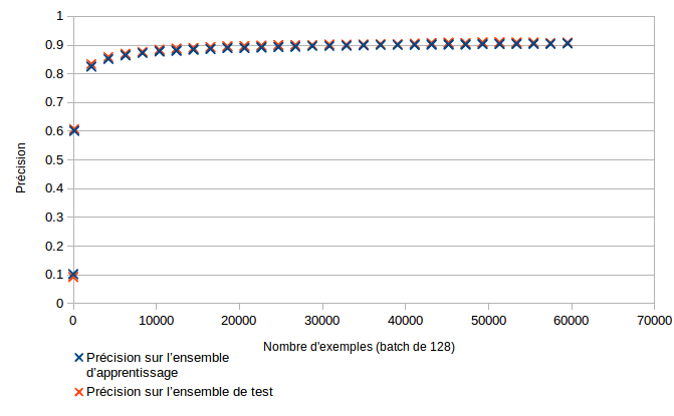
\includegraphics[scale=0.5]{images/mnist_apprentissage_128.png}
\caption{Précision en fonction du nombre d'exemples appris}
\label{mnist_apprentissage_128}
\end{center}
\end{figure}

On peut remarquer sur ces premiers résultats, que la précision progresse très vite avant de plafonner autour des 90\% dès les 10.000 exemples utilisés. Nous avons obtenu une précision maximale de 90.83\% sur cette architecture neuronale, très simpliste. Une précision plus importante pourrait être obtenue en ajoutant au moins une couche cachée au réseau. Cependant, le temps d'exécution avec cette première architecture (21.565 secondes soit plus de 6 heures), nous a montré que cela serait impossible avec de réaliser un apprentissage en un temps raisonnable avec des architectures plus compliquées.
\label{resultat_premiere_implementation}


\section{Conclusion}
Cette première implémentation intuitive permet ainsi d'obtenir des résultats très satisfaisants, allant jusqu'à 90\% de réussite sur MNIST. De plus, elle met en évidence le fonctionnement d'un réseau de neurones. Cependant, on remarque que les calculs ne sont pas du tout optimisés. Cela explique que le temps d'exécution devient rapidement très long. Dans l'exemple de l'application à l'ensemble de données MNIST, entraîner plusieurs fois le réseau sur l'ensemble d'apprentissage permettrait d'obtenir de bien meilleurs résultats, mais cela prendrait alors beaucoup trop de temps pour être véritablement envisageable.
Afin d'améliorer le temps de calcul et d'optimiser l'algorithme, nous nous sommes intéressés à une nouvelle approche des réseaux neuronaux basée sur les Computational Graphs, ou Graphes de calculs.

\chapter{Graphe de calculs}

\section{Définition}

Nous avons vu précédemment que l'architecture du réseau de neurones peut être lourde autant du point de vue modélisation que du point de vue calcul. Pour motiver l'apparition des graphes de calcul prenons l'exemple d'un réseau de neurones à $m$ entrées possèdant une seule couche de $n$ neurones ayant pour fonction d'activation une sigmoïde $\sigma$.

Nous pourrions modéliser ce réseau de neurone en définissant $n$ neurones ayant chacun son vecteur poids mais une façon équivalente de modéliser ce système est de rassembler tous les poids dans une matrice $W \in \mathbb{R}^{m \times n}$. En notant $x \in \mathbb{R}^m$ le vecteur ligne des entrées du réseau, on a alors que la sortie est :
$$y = \sigma(xW)$$
où la fonction $\sigma$ s'applique terme à terme. 

Cette manière de modéliser a plusieurs avantages. Tout d'abord, elle est plus compacte et simple à manipuler. Puis, elle a un avantage certain pour notre implémentation en Python car elle permet d'utiliser pleinement la librairie d'algèbre linéaire \texttt{numpy} ce qui accélerera grandement les calculs. Enfin, il est facile d'étendre la formule précédente au calcul de la sortie de plusieurs vecteurs d'entrées. En effet si $X \in \mathbb{R}^{l \times m}$ est une matrice contenant $l$ vecteurs d'entrées alors la sortie du réseau s'écrit :
$$Y = \sigma(XW)$$

On aurait donc envie de s'affranchir de la structure du neurone pour seulement modéliser les opérations mathématiques effectuées par le réseau.

Un graphe de calcul est simplement un graphe représentant une formule mathématique. Un n\oe{}ud de ce graphe représente soit une constante, une variable, des poids ou une opération mathématique.

Par exemple, le graphe de calcul représente le réseau présenté ci-dessus est :

% Insérer le graphe du réseau

Finalement, nous ne sommes même pas obligés de rester cantonnés à des graphes de calculs représentant des réseaux de neurones,  nous pouvons modéliser un beaucoup plus grand ensemble de fonctions mathématiques grace à ce formalisme.

\section{Dérivation automatique}

Nous avons modéliser nos réseaux de manière plus efficace. Il reste cependant un problème à résoudre. Nous avons besoin de calculer la dérivée du coût $E$ par rapport aux poids avant de pouvoir utiliser l'algorithme de la descente du gradient.

Afin de réaliser cela, nos n\oe{}uds représentant des opérations mathématiques ne seront pas seulement responsable de calculer une sortie mais aussi de propager une erreur.

\section{N\oe{}uds}


\section{Legacy}

Un graphe de calcul est la représentation de fonctions composées comme un réseau d’entités interconnectés. Chacune de ces entités est une fonction ou une opération, cela permet alors une meilleure visualisation de la tâche globale effectuée par le réseau ainsi que les relations entre deux neurones successifs. On appellera par la suite nœud parent un nœud situé en amont du réseau (i.e. plus proche des inputs) par rapport à un autre (appelé alors nœud enfant) et en lien direct avec lui. 

L’intérêt principal de cette représentation est la rapidité et la facilité de l’implémentation de l’algorithme de backpropagation. En effet, le caractère modulaire de cette dernière rend aisé le calcul de gradient en appliquant la règle de la chaîne, comme le montre l’exemple suivant :

\begin{figure}[!h]
\begin{center}
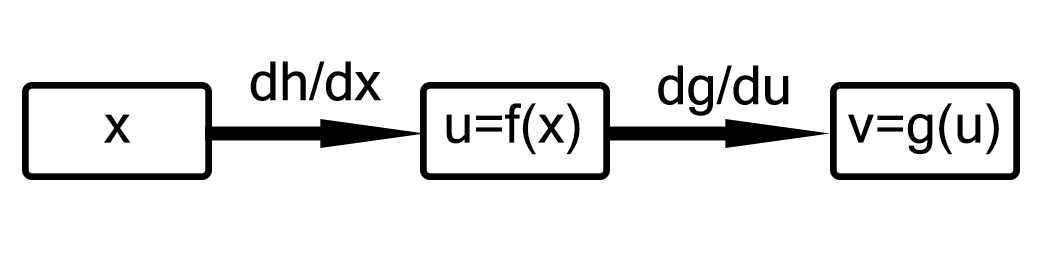
\includegraphics[scale=0.25]{images/retropropagation_graphe.png}
\caption{Décomposotion de la rétropropagation de l'erreur dans un graphe de calcul simple.}
\label{retropropagation_graphe}
\end{center}
\end{figure}

Supposons que l’on veuille sur cet exemple simple obtenir la dérivée de g par rapport à x, il suffira alors de faire le produit des dérivées indiquées sur chaque branche connectant deux nœuds différents.

\section{Diagramme UML}

Là encore, l'architecture retenue contient 2 classes mères : Node et Graph, un graph étant constitué de plusieurs nodes qui connaissent chacune leurs parents et leurs enfants.

La différence principale avec l'architecture précédente est dans la modularité de la classe Node. Bien qu'elle joue un rôle similaire à celui de la classe Neuron dans le modèle Neuron/Network, elle est bien plus souple : une node peut représenter une entrée du graph, un vecteur de poids, une opération élémentaire (addition, soustraction, produit scalaire), ou une fonction (fonction d'activation d'un neurone ou fonction de coût du réseau). Une node prend pour entrée une matrice (ou 2 dans le cas des opérateurs élémentaires), et donne en sortie ses résultats sous la forme d'une matrice de taille adaptée. De même elle peut calculer le gradient par rapport à ses entrées étant donné celui de ses enfants toujours sous forme matricielle.  Cette capacité des nodes à gérer les matrices est primordiale car elle permet de créer un réseau ne possédant qu'une seule node d'entrée et de propager à travers lui tout un lot d'exemples en une seule fois, diminuant ainsi grandement le nombre d'appels objet en les remplaçant par des opérations matricielles. Les résultats obtenus avec cette architecture permettront par la suite de confirmer que les appels objets et non les opérations occupaient la majeure partie du temps de calcul dans l'implémentation présentée en chapitre 1.

\begin{figure}[!h]
\centering

\tikzset{every picture/.style={scale=0.6}}
\begin{tikzpicture}[line cap=round,line join=round,>=triangle 45,x=1.0cm,y=1.0cm, scale=0.5]
\clip(2.4143827288284365,2.1911915106170423) rectangle (28.896515457132203,16.893403649017483);
\draw(4.982,6.946) circle (1.5319647515527244cm);
\draw(10.46,6.946) circle (1.5319647515527248cm);
\draw(15.918356266000036,6.947742334000014) circle (1.5319647515527248cm);
\draw(21.396356266000033,6.947742334000014) circle (1.531964751552723cm);
\draw(26.874356266000035,6.947742334000014) circle (1.531964751552723cm);
\draw (4.683242626729719,7.418644715381643) node[anchor=north west] {$\mathcal{X}$};
\draw (10.001450227410324,7.781662299045852) node[anchor=north west] {$\times$};
\draw (15.119998157075615,7.509399111297696) node[anchor=north west] {$z=f(y)$};
\draw(15.911114126755379,11.67271742202839) circle (1.531964751552723cm);
\draw (14.575471781579308,10.141276592863207) node[anchor=north west] {sortie attendue};
\draw (14.212454197915102,5.222388334213182) node[anchor=north west] {fonction d'activation};
\draw (7.859646483791514,5.167935696663551) node[anchor=north west] {opération élémentaire};
\draw (4.10241449286699,5.1316339382971305) node[anchor=north west] {Entrée};
\draw (19.966282898992755,5.167935696663551) node[anchor=north west] {fonction de coût};
\draw (20.420054878573012,7.563851748847327) node[anchor=north west] {$c=h(z,y')$};
\draw (15.646373653388713,12.228627698932405) node[anchor=north west] {y'};
\draw (25.30264137885657,5.186086575846762) node[anchor=north west] {gradient constant};
\draw [->] (6.511832012049577,6.86519149235171) -- (8.930169512469373,6.865162635979358);
\draw [->] (12.00521159541307,6.880938976773743) -- (14.423549095832865,6.880910120401391);
\draw [->] (17.483211595413067,6.880938976773743) -- (19.901549095832866,6.880910120401391);
\draw [->] (22.92499832258255,6.977574257545156) -- (25.34333582300235,6.9775454011728035);
\draw(4.9814182705273335,11.336093947857117) circle (1.5319647515527193cm);
\draw (4.429130318164775,9.760108130015787) node[anchor=north west] {$poids$};
\draw (4.719544385096139,11.883760994451407) node[anchor=north west] {$w$};
\draw [->] (6.513382260277414,11.334566168750113) -- (8.905056271433413,6.865162935638539);
\draw [->] (17.442307496209068,11.624108108712399) -- (19.901549095832852,6.880910120401391);
\end{tikzpicture}
\caption{Schéma d'un graphe de calcul pour un neurone simple}
\label{graphe_de_calcul}
\end{figure}

Un graph commence par une node d'entrée, suivie d'un ensemble de nodes de calcul dont la dernière est qualifiée de node de sortie. Une ou plusieurs node(s) de fonction de coût prennent pour parent la node de sortie, une node d'entrée qu'on actualisera aux valeurs des sorties attendues lors de l'entrainement et une node de régularisation. Enfin on clôt le graph par une node qui possède un gradient unitaire constant et aucune sortie. Elle permettra d'initier la descente du gradient dans la pile des appels récursifs des nodes depuis les entrées vers la fin du graph. C'est le graph qui gère la propagation des exemples et la descente du gradient à travers les nodes mais son rôle est très limité de par la grande autonomie qui est donnée à celles-ci. Les fonctions de propagation et rétropropagation de chaque node sont en effet codée de sorte à ce qu'un unique appel de leur fonction de propagation (respectivement rétropropagation) sur la node d'entrée (respectivement de sortie) donne lieu à une cascade d'appel jusqu'à l'obtention du résultat voulu. Dans une propagation par exemple, on appelle la méthode « propager » sur la dernière node du réseau qui l’appellera elle-même sur ses parents pour calculer sa sortie, ce qui actualisera les sorties de toutes les nodes nécessaires au calcul du résultat initialement demandé.



\section{Résultats}

L'architecture en Graphe de Calcul donne de très bons résultats du point de vue de la rapidité de calcul. On observe par exemple une réduction d'un facteur 1000 du temps de calcul pour l'entrainement du réseau simple sur l'ensemble MNIST par rapport à l'implémentation "naïve" du chapitre 1. Ces performances sont atteintes grâce à la diminution du nombre d'appels objets, remplacés par des calculs matriciels sur des matrices de grande taille gérées par des bibliothèques efficaces.

\chapter{Études des paramètres}

\section{Approche du problème}

L'implémentation basée sur les graphes de calcul nous a permis de réaliser des tests sur les deux exemples introduits précédemment : XOR et MNIST. \`A travers de nombreux tests, nous avons souhaité étudier l'influence des paramètres de l'algorithme sur ses performances, c'est-à-dire sur sa précision et sa rapidité.
\medbreak
Il existe sept paramètres que l'on peut définir pour un réseau de neurones :
\begin{itemize}
\item l'architecture du réseau
\item le prétraitement des données
\item l'initialisation des poids
\item le choix des fonctions d'activations
\item le choix de la fonction de coût
\item la taille des batchs et le nombre de passage
\item le taux d'apprentissage
\end{itemize}
\medbreak
L'influence d'un paramètre n'étant bien évidemment pas indépendante ni des autres paramètres ni du problème considéré, il devient rapidement délicat d'obtenir des résultats robustes. En effet, il est impossible de réaliser des mesures en faisant varier sept variables en même temps, tout en effectuant des répétitions à chaque fois pour s'assurer de la précision des relevés. Pour s'affranchir de cette difficulté, nous avons choisi de ne faire varier qu'un seul paramètre à la fois en l'intégrant dans une configuration apportant des résultats acceptables. L'influence du paramètre étudié sur plusieurs configurations permet alors d'interpoler une estimation de son comportement général.
C'est donc ainsi que nous avons pu déterminer des éléments permettant de comprendre les rôles de ces paramètres et de les choisir pour optimiser l'efficacité d'un réseau de neurones. Ce sont ces éléments qui vont être présentés dans la suite de cette partie.

\section{\'Etude du XOR}

Dans un premier temps, nous avons effectués plusieurs tests sur un exemple très simple : XOR.
Quelques résultats ont déjà été présentés en partie \ref{resultat_premiere_implementation}. Ils vont être rapelés et détaillés dans cette partie.

\begin{figure}[!h]
\begin{center}
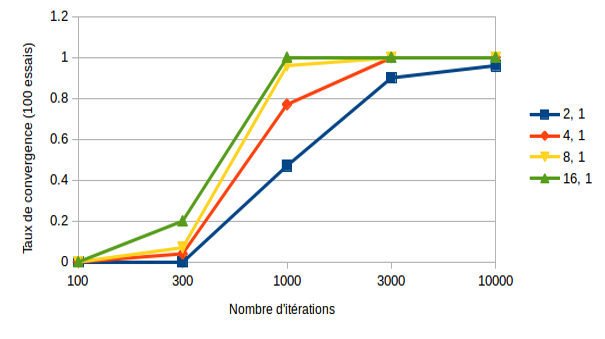
\includegraphics[scale=0.6]{images/xor_architecture_tanh.png}
\caption{Convergence en fonction de l'architecture avec tanh}
\label{xor_architecture_tanh}
\end{center}
\end{figure}

\begin{figure}[!h]
\begin{center}
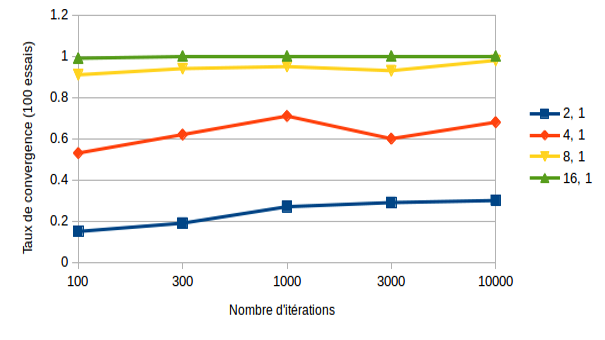
\includegraphics[scale=0.6]{images/xor_architecture_relu.png}
\caption{Convergence en fonction de l'architecture avec relu}
\label{xor_architecture_relu}
\end{center}
\end{figure}

\begin{figure}
\begin{center}
\begin{tabular}{cc}
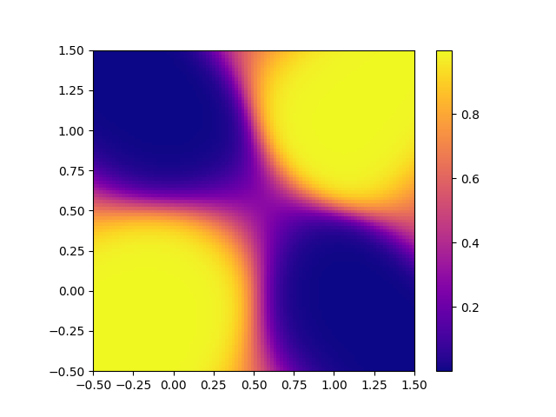
\includegraphics[scale=0.5]{images/xor_tanh_centre.png} & 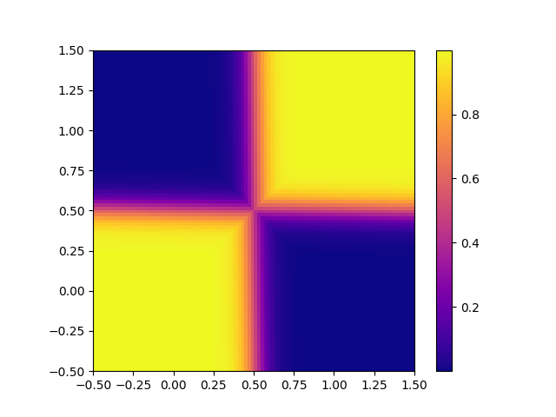
\includegraphics[scale=0.5]{images/xor_relu_centre.png} \\
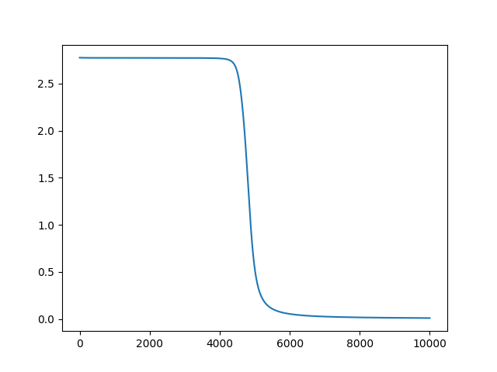
\includegraphics[scale=0.5]{images/cout_xor_tanh_centre.png} & 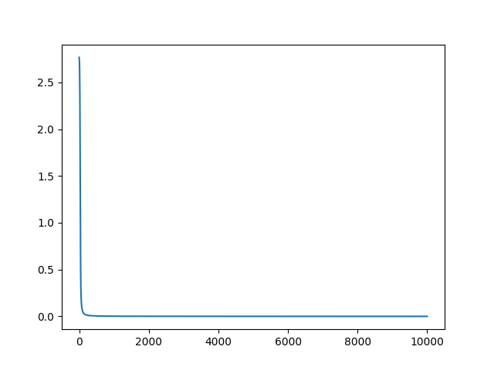
\includegraphics[scale=0.5]{images/cout_xor_relu_centre.png}
\end{tabular}
\caption{Résultat après centrage des entrées pour tanh (à gauche) et pour relu (à droite)} 
\label{differentes_fonctions_activation}
\end{center}
\end{figure}


\section{\'Etude de MNIST}
\subsection{Architecture du réseau}
Le nombre de couches cachées d'un réseau de neurone ainsi que leur composition constitue l'architecture de ce réseau.


\subsection{Prétraitement des données}


\subsection{Initialisation des poids}
Avant le lancement de l'algorithme sur un réseau de neurone, il est nécessaire d'initialiser les poids.	L'usage le plus courant est de les initialiser aléatoirement. Cependant, le choix de la distribution aléatoire n'est pas forcément évident. En effet, on peut choisir d'utiliser une distribution uniforme, une distribution gaussienne ou tout autre type de distribution aléatoire avec des paramètres variables.

Nous avons donc testé trois types de fonction d'initialisation des poids : une répartition uniforme, une répartition uniforme centrée en 0  et une répartition gaussienne centrée en 0.
Si les initialisations centrées en 0 permettent une convergence un petit peu plus rapide, ces trois initialisations produisent des résultats similaires. Cependant, l'amplitude des poids change beaucoup les résultats quelle que soit la fonction d'initialisation. En effet, les poids convergeant lors de l'apprentissage vers de petites valeurs, une initialisation avec de petites amplitudes va permettre une convergence plus rapide.

\begin{figure}[!h]
\begin{center}
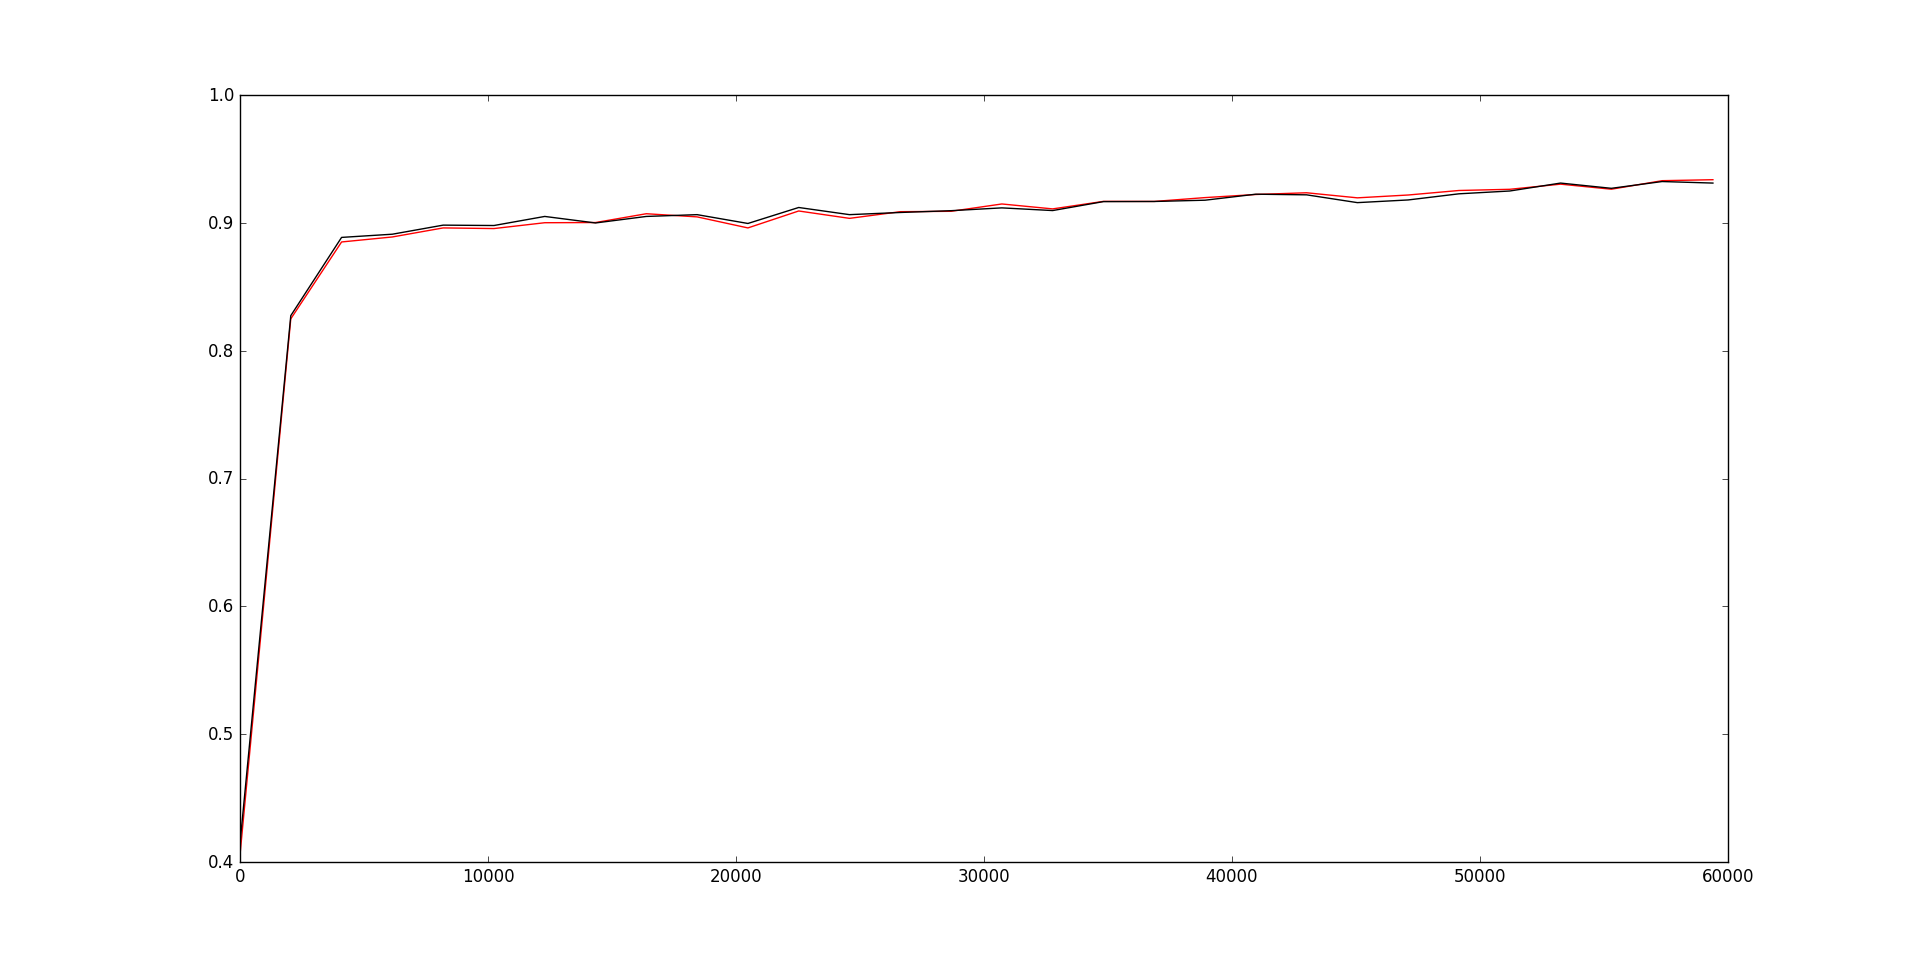
\includegraphics[scale=0.2]{images/initialisationpoids_amplitude01.png}
\caption{Précision sur les ensembles de test (en noir) et d'apprentissage (en rouge) en fonction du nombre d'exemples utilisés pour l'apprentissage pour une initialisation des poids d'amplitude 0.1 }
\label{initialisationpoids_amplitude0.1}
\end{center}
\end{figure}

\begin{figure}[!h]
\begin{center}
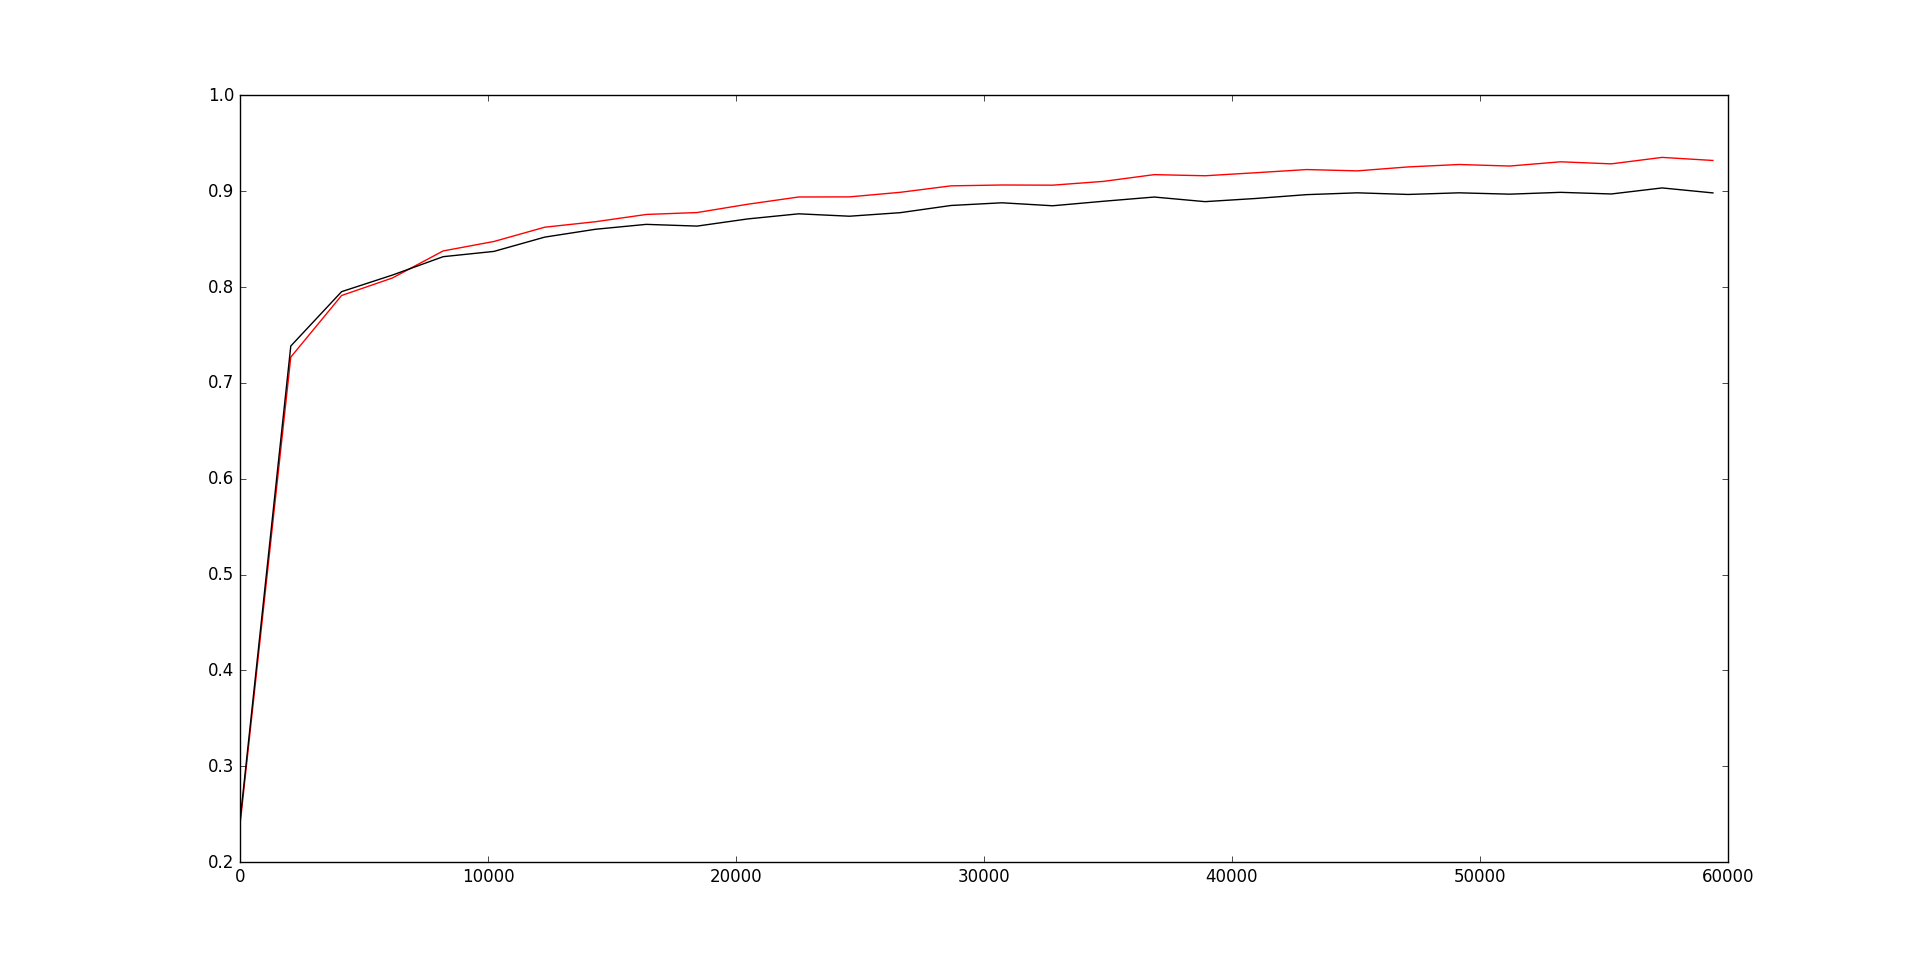
\includegraphics[scale=0.2]{images/initialisationpoids_amplitude10.png}
\caption{Précision sur les ensembles de test (en noir) et d'apprentissage (en rouge) en fonction du nombre d'exemples utilisés pour l'apprentissage pour une initialisation des poids d'amplitude 0.1}
\label{initialisationpoids_amplitude10}
\end{center}
\end{figure}

C'est ce que l'on peut voir sur les deux figures \ref{initialisationpoids_amplitude0.1} et \ref{initialisationpoids_amplitude10}. Dans les deux cas, les poids sont initialisés selon une loi normale centrée de variance 0,1. Cependant, sur la première, un coefficient multiplicatif de 0,1 leur est affecté alors que celui-ci est de 10 sur la deuxième.
On peut ainsi bien observer que dans le cas du facteur multiplicatif de 10, la convergence est plus lente au début de l'apprentissage, même si l'on atteint sensiblement les mêmes valeurs finales de précision.



\subsection{Choix des fonctions d'activations}


\subsection{Choix de la fonction de coût}


\subsection{Taille des batchs et nombre de passages}


\subsection{Taux d'apprentissage}
Nous avons aussi étudié l'influence du taux d'apprentissage ou learning rate. En effet celui-ci influe sur la mise à jour des poids : plus il est grand et plus chaque l'importance donnée au calcul de la dérivée est important. Avoir un taux d'apprentissage grand permet d’obtenir rapidement des performances satisfaisantes en termes de précision. Au contraire, des phénomènes d'oscillations sont observés pour un apprentissage conséquent, et cela fournit en retour de moins bons résultats, par rapport à des taux d'apprentissage plus faibles. Cela a été illustré sur la figure \ref{influence_learningrate}.

\begin{figure}[!h]
\begin{center}
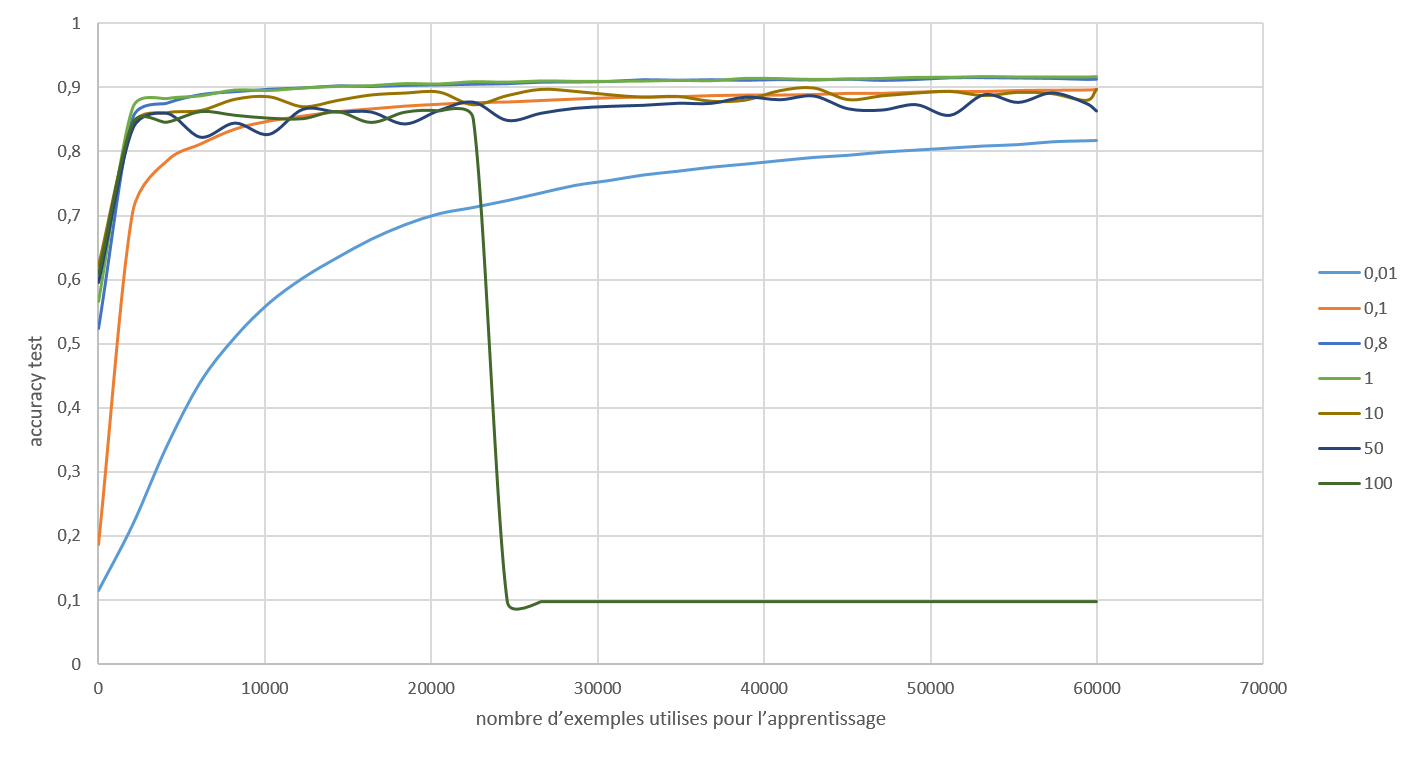
\includegraphics[scale=0.6]{images/influence_learningrate.png}
\caption{Influence du learning rate sur la précision sur l'ensemble de test en fonction du nombre d'exemple utilisés}
\label{influence_learningrate}
\end{center}
\end{figure}

L'architecture du réseau a été choisie sans couche cachée avec 10 neurones de sortie sous forme de Softmax. Le neurone de coût est un SoftmaxCrossEntropy, et l'apprentissage se fait avec des lots de 128 exemples. Nous avons alors étudié l'apprentissage du réseau pour des taux d'apprentissage allant de 0.01 à 100.
Nous pouvons alors distinguer trois cas reflétant les principaux comportements :

\begin{itemize}

\item Pour un taux d'apprentissage de 0.01, la convergence est très lente mais sans oscillations. Si la précision obtenue peut-être à hauteur des autres taux d'apprentissage en utilisant plus d'exemples, on peut considérer celui-ci trop petit.
\item Pour un taux d'apprentissage de 100, la convergence est très rapide au début, mais oscille beaucoup et va finalement bloquer l'apprentissage vers un autre minimum local de coût non désiré. On peut donc considérer ce taux d'apprentissage comme trop grand.
\item Pour un taux d'apprentissage de 0.1, il semble apparaître un bon compromis entre stabilité et vitesse de la convergence. C'est cette valeur qui en général sera choisie pour les tests, bien que d'autres soient satisfaisants (0.8 ou 1 par exemple).

\end{itemize}

\chapter{Réseaux de neurones récurrents}
\section{Motivation}
Nous avons pu voir que les réseaux feedforward peuvent être utilisés afin d'appendre à générer la sortie voulu en fonction de l'entrée du réseau. 
Néanmoins, ces réseaux sont limités à des entrées et des sorties de tailles fixes. De plus il ne peuvent gérer des réseaux présentant des cycles. On utilise alors des réseaux récurrents qui permettent un traitement plus efficace des séquences de données. On pourra ainsi prévoir la suite d'une séquence.

Nous nous intéresserons à deux algorithmes permettant l'apprentissage des réseaux récurrents : Real Time Recurrent Learning (RTRL) et Back Propagation Through Time (BPTT).

\section{Dépliage}

Nous avons dit précédemment qu'un réseau de neurones récurrent est un réseau possédant des cycles. Néanmoins, il est difficile d'imaginer que la valeur de sortie d'un neurone au temps $t$ dépende de la sortie de ce même neurone au temps $t$. Pour résoudre ce problème, nous allons ajouter une dimension temporelle à nos réseaux et permettre aux neurones au temps $t$ de dépendre des valeurs d'autres neurones au temps $t-1$.

Afin de mettre en évidence cette dépendance temporelle sur nos graphes, les arêtes reliant la sortie d'un neurone au temps $t-1$ à un neurone au temps $t$ vont être annontées par un carré comme sur la figure \ref{arete_retard}. On les appelera arête "retard".

% Insérer figure avec une arête retard

On a alors de nouvelles équations pour la sortie du neurone $j$ :
\begin{equation}
\left\{
\begin{array}{ll}
t = 0, & y_j(t) = 0 \\
\forall t \geq 1, & y_{j}(t) = g_{j}(\sum_{i \in Pa_t(j)}{w_{ji}y_{i}(t)} + \sum_{i \in Pa_{t-1}(j)}{w'_{ji}y_{i}(t-1)})
\end{array}
\right.
\end{equation}
où $Pa_t(j)$ est l'ensemble des neurones ayant une arête allant vers $j$ au temps $t$ et $Pa_{t-1}(j)$ l'ensemble des neurones ayant une arête "retard" allant vers $j$.

Une manière commode de mettre en évidence cette dépendance temporelle est de déplier le graphe. 

% Insérer figure avec les instants t-1, t et t+1 d'un réseau

On peut même pour une séquence d'entrée donnée modéliser tous les calculs du réseau sans aucun cycle si on déplie le réseau un nombre suffisant de fois.

% Insérer figure avec le réseau déplier pour une séquence d'entrée


\section{RTRL}

\section{BPTT}

\section{Évaluation}

\subsection{Grammaire de Reber}

Dans un premier temps, nous comparerons ces algorithmes sur l'apprentissage de la grammaire de Reber, qui est régulière. Nous utiliserons la grammaire simple présentée sur la figure \ref{Grammaire de Reber simple}.

\begin{figure}[h!]
\begin{center}
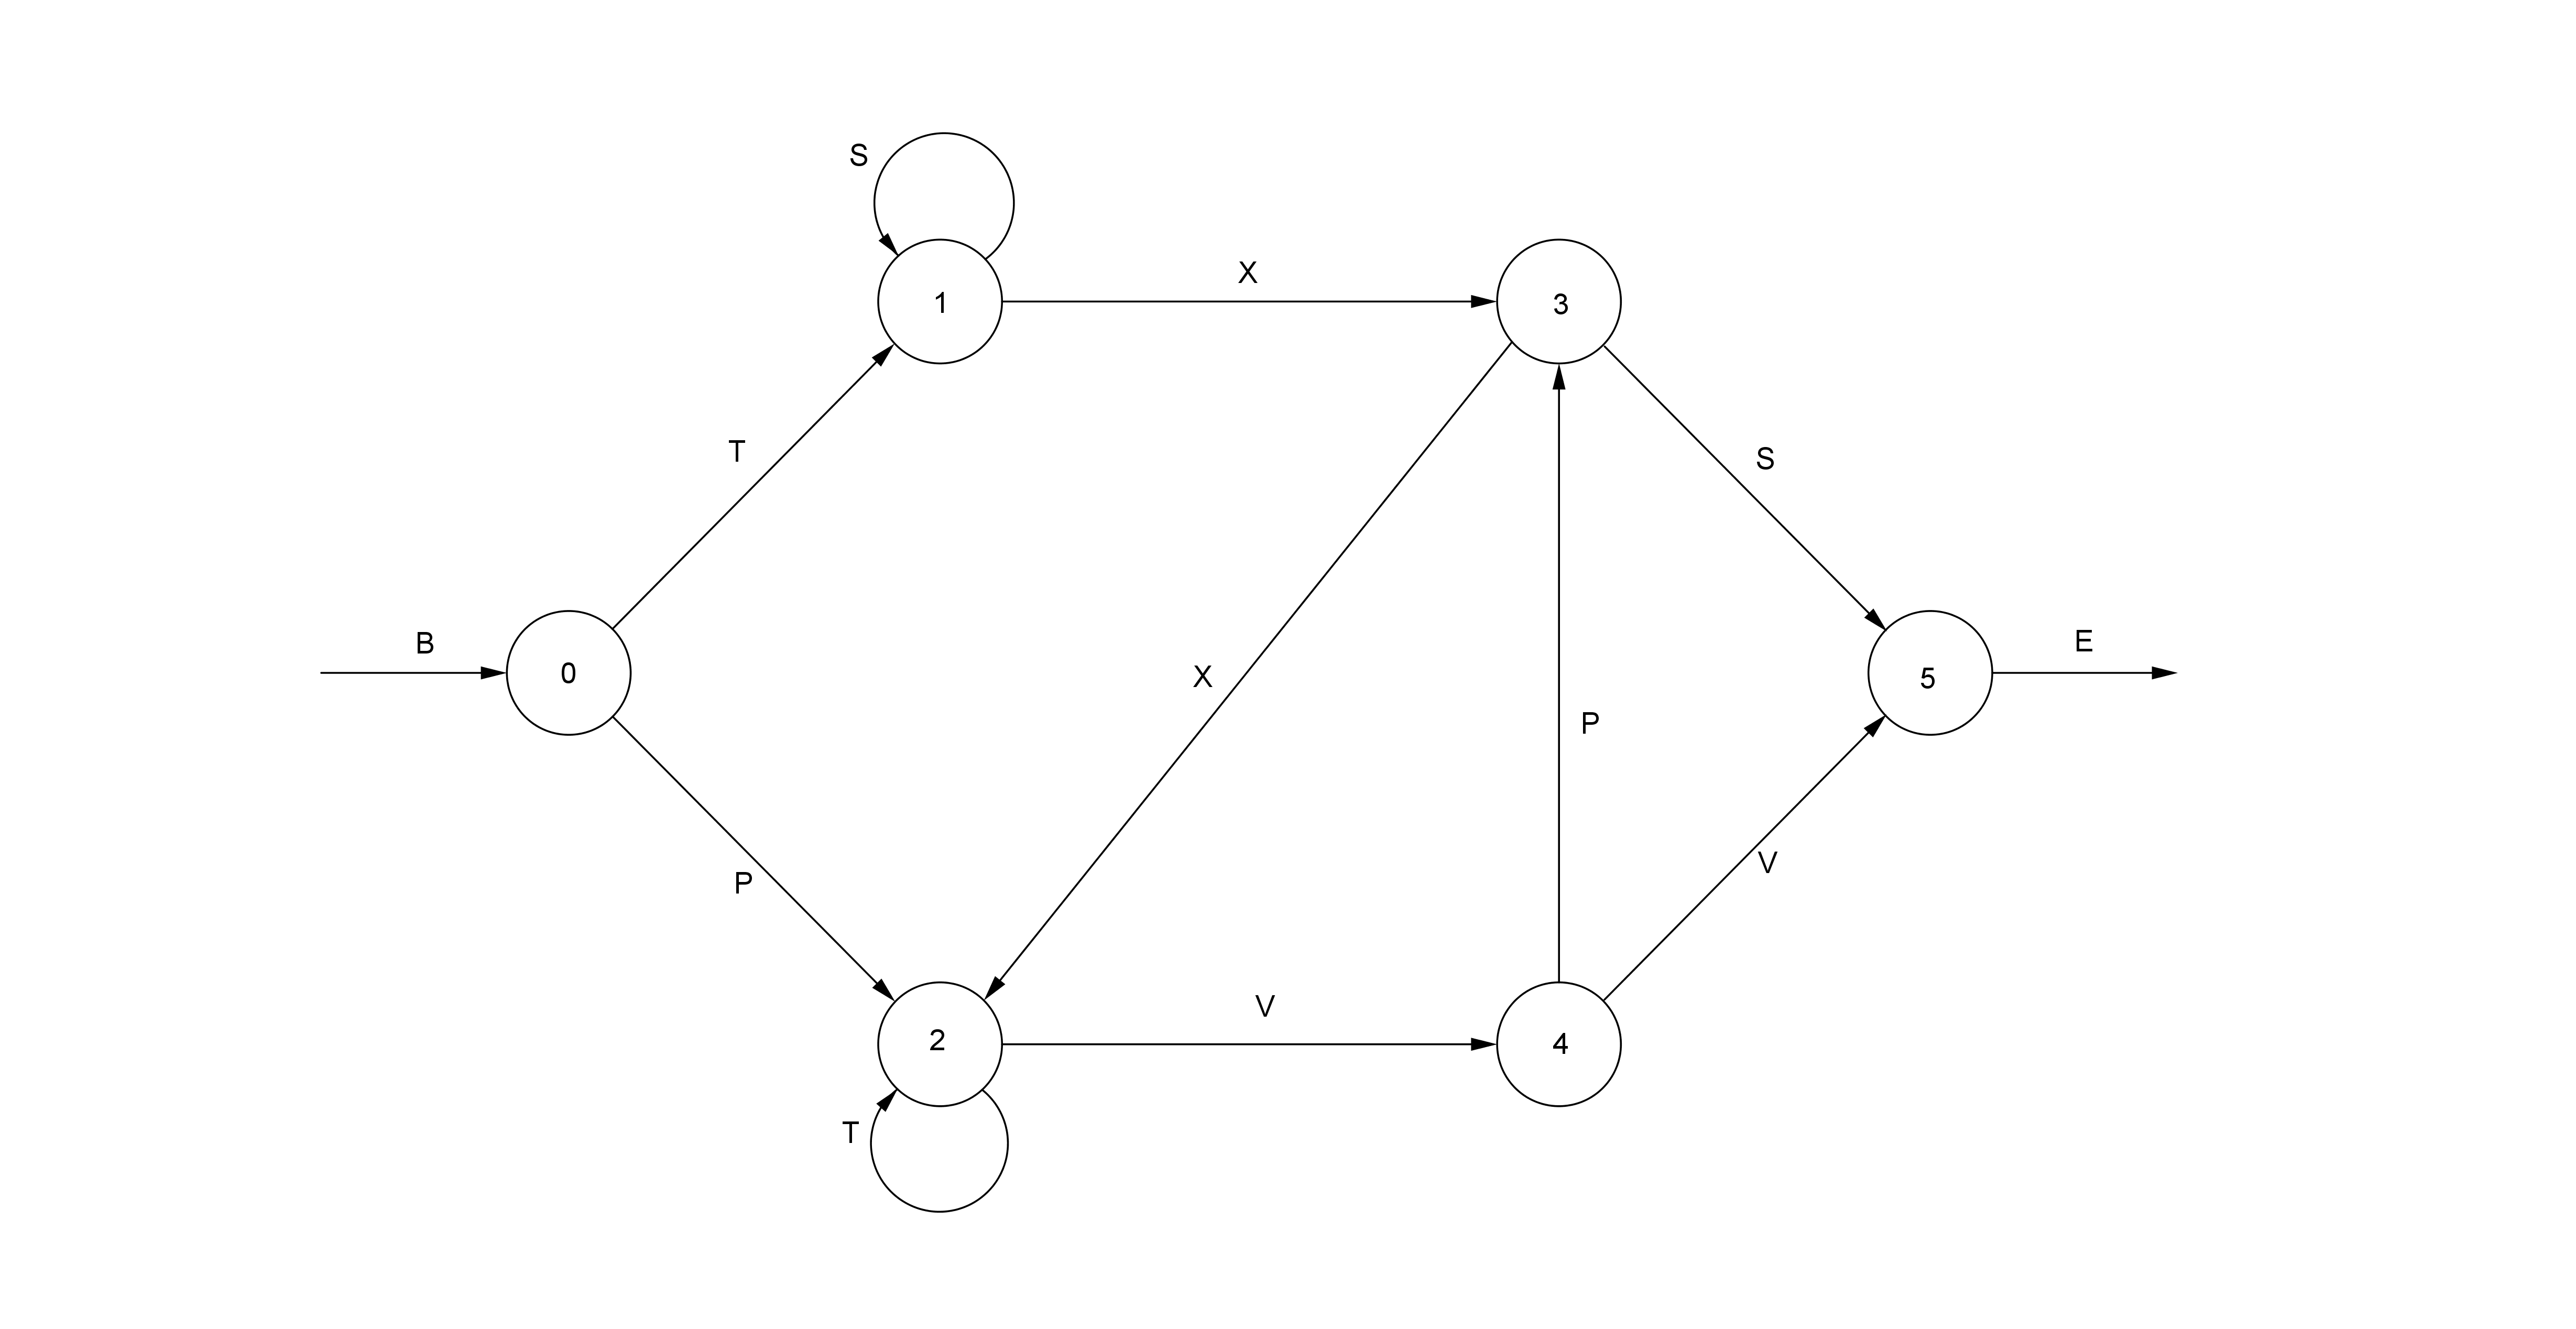
\includegraphics[scale=0.3]{images/reber_simple.png}
\caption{Automate reconnaissant la grammaire de Reber simple}
\label{Grammaire de Reber simple}
\end{center}
\end{figure}

A l'aide de cette automate, nous générerons deux ensembles de mots respectivement afin d'entraîner et de tester notre futur réseau. L'objectif du réseau sera alors d'apprendre cette grammaire afin de prédire les caractères possibles après un caractère donné.

L'étape suivante consistera à tester les algorithmes sur l'apprentissage de la grammaire de Reber symmétrique présentée sur la figure \ref{Grammaire de Reber symmétrique}.  
\begin{figure}[h!]
\begin{center}
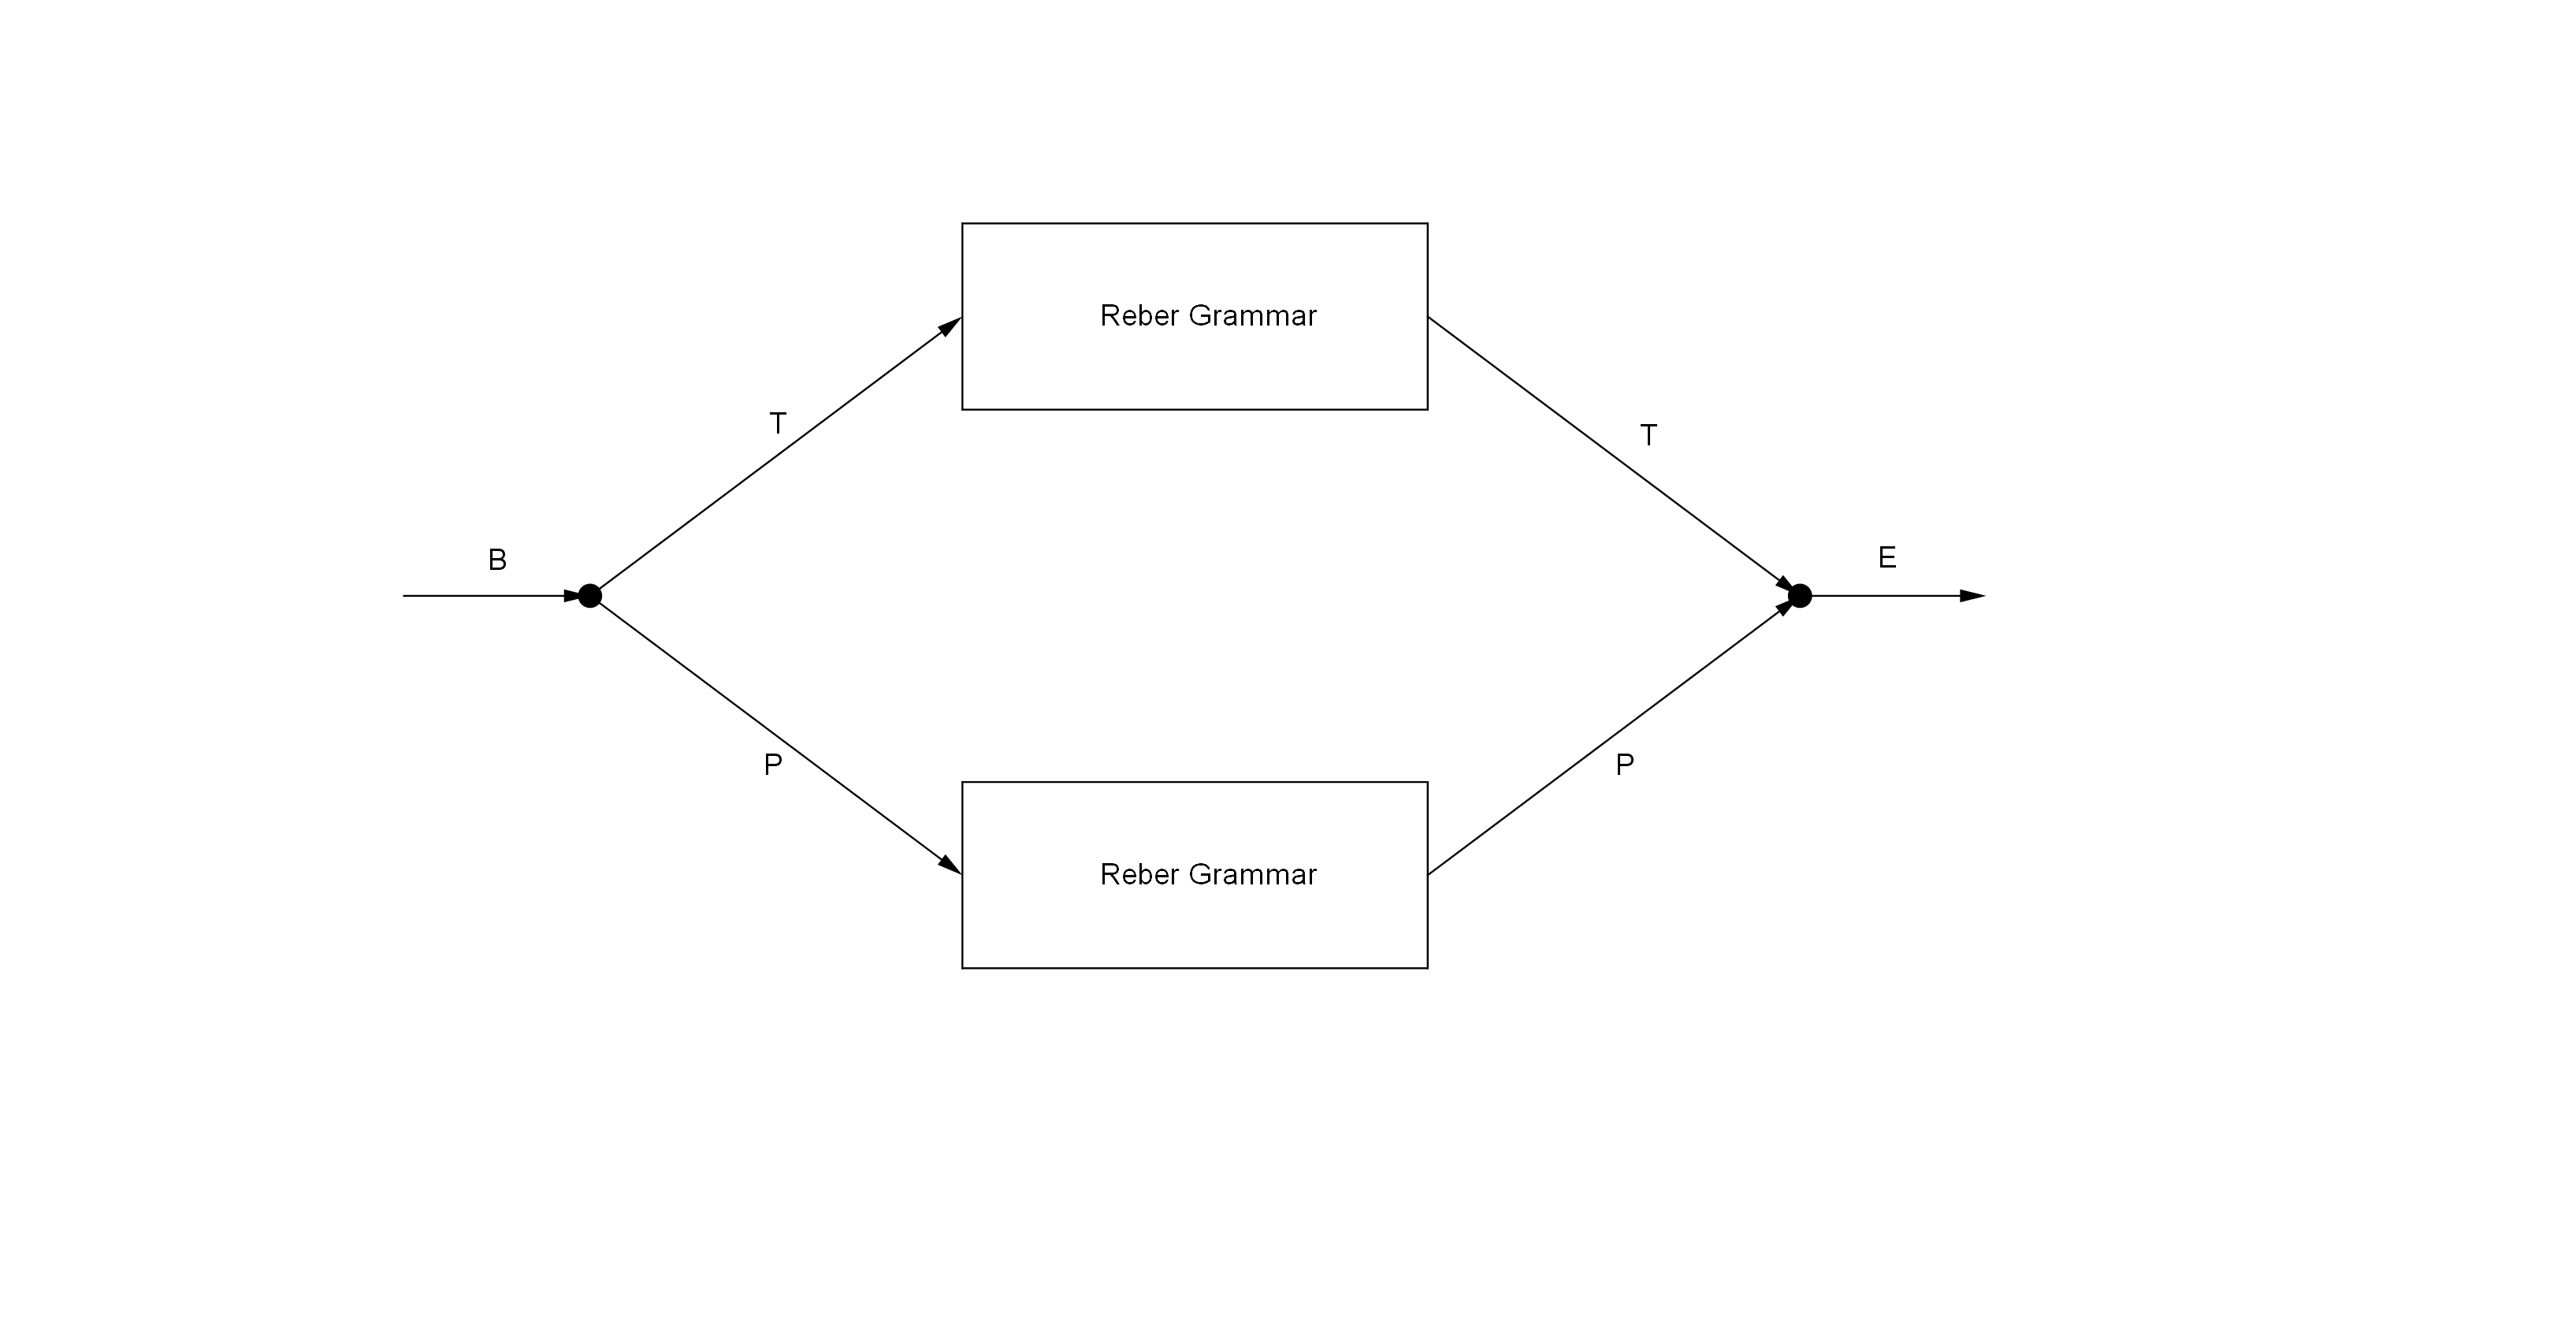
\includegraphics[scale=0.5]{images/reber_symmetrique.png}
\caption{Automate reconnaissant la grammaire de Reber symmétrique}
\label{Grammaire de Reber symmétrique}
\end{center}
\end{figure}

Dans cette situation, le réseau devra être capable de se souvenir d'un état passé (T ou P) afin de prédire le nouvel état (T ou P). Cet état passé pourra être plus ou moins lointain en fonction de la taille de la grammaire de Reber insérée au milieu. 
\bigbreak
\bigbreak

\subsection{Shakespeare}

Enfin, nous appliquerons ces deux algorithmes à l'apprentissage de textes de Shakespeare. L'objectif sera alors de générer un texte anglais cohérent.

\section{Comparaison des deux algorithmes}

\chapter{Long Short-Term Memory (LSTM)}
\section{Motivation}
Les réseaux de neurones récurrents étudiés jusqu'alors permettent effectivement d'apprendre des suites de séquences. Néanmoins, on observe un phénomène d'oubli se caractérisant par une faible influence des plus vieilles informations sur la sortie actuelle.

Cela est dû à la rétropropagation du gradient. En effet, celle-ci est basée sur la règle de la chaîne qui fait donc apparaître un produit de dérivées de fonctions d'activation. Or si ces dérivées sont supérieures à 1, cette partie du gradient rétropropagé risque d'exploser. A l'inverse, si elles sont inférieures à 1, comme c'est le cas pour la sigmoide dont la dérivée a une valeur maximale de 0
25, cette partie du gradient tend à disparaître lorsque l'on remonte loin dans le temps. Ainsi, on perd la dépendance à long terme.

Nous travaillions jusque là avec des réseaux récurrents comme celui présenté sur la figure \ref{RNN classique} composé d'une simple couche de tangentes hyperboliques.

\begin{figure}[h!]
\begin{center}
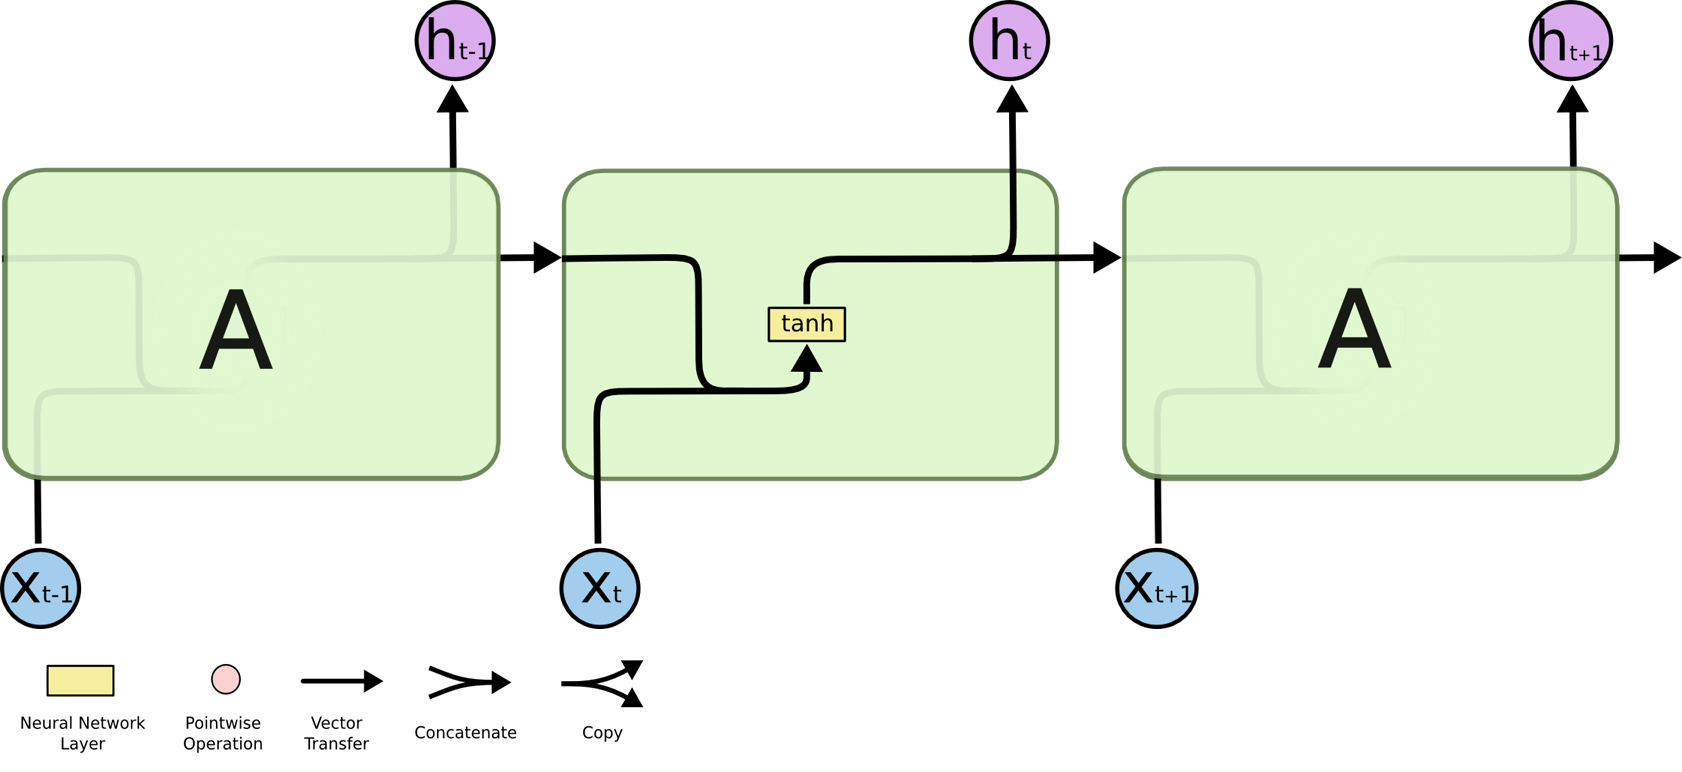
\includegraphics[scale=0.25]{images/RNN_classique.png}
\caption{Dépliage d'un RNN classique}
\label{RNN classique}
\end{center}
\end{figure}

Dans le cadre des LSTM, nous utilisons une nouvelle cellule de base afin d'éviter cette disparition du gradient lors de la rétropropagation.

\newpage

\section{Principe de fonctionnement}
Comme pour les réseaux récurrents, on peut déplier les LSTM afin de se ramener à une cellule de base qui se répète. Le principe des LSTM repose sur l'existence d'un état qui apparaît tout en haut de la cellule et qui subit seulement quelques modifications linéaires. Cela permettra ainsi, lors de la rétropropagation du gradient, de ne pas perdre la dépendance avec les informations lointaines.

La cellule de base des LSTM peut donc être représentée par la figure suivante.

\begin{figure}[h!]
\begin{center}
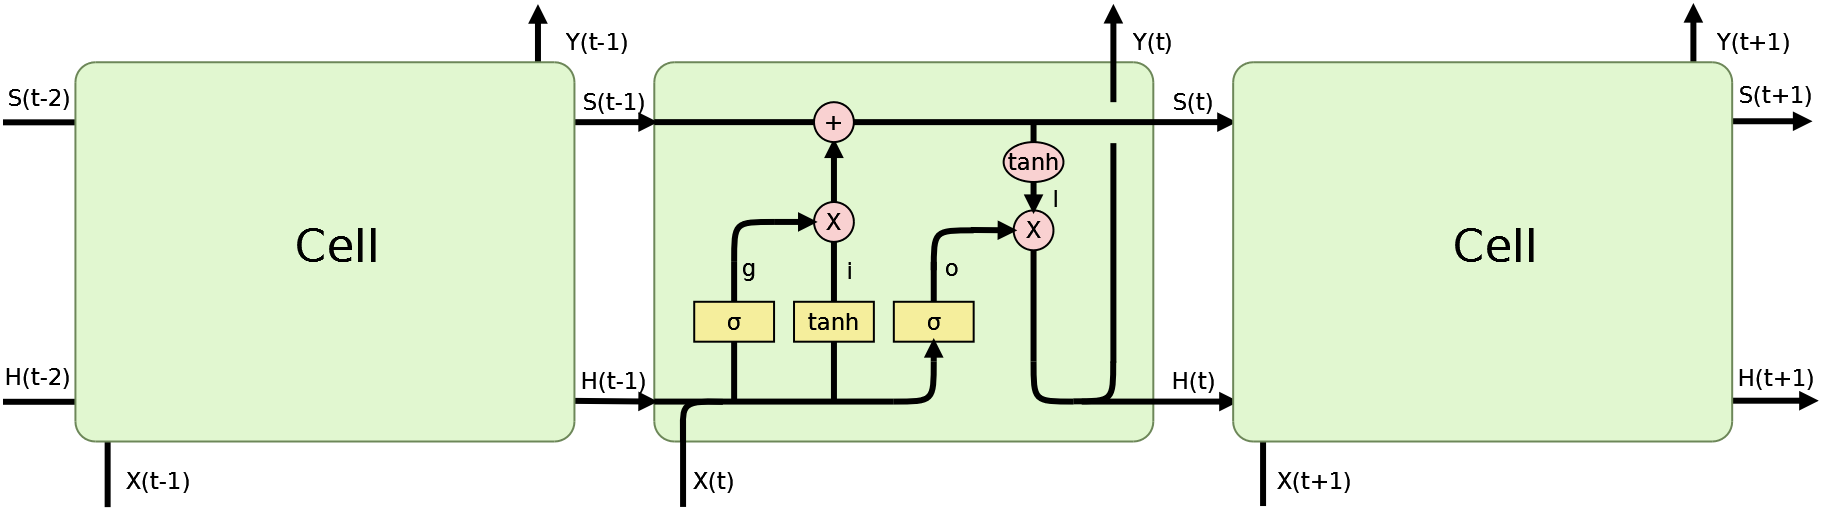
\includegraphics[scale=0.12]{images/LSTM_article_plusieurscell.png}
\caption{Cellule élémentaire des LSTM}
\label{cellule LSTM}
\end{center}
\end{figure}

Cette figure permet de représenter facilement le réseau en utilisant la structure d'un graphe de calcul. Il faut cependant bien distinguer les fonctions tanh et sigmoide qui symbolisent une couche entière de neurones (dans les rectangles jaunes) et la fonction tanh (dans le cercle rose) qui s'applique à chaque élément du vecteur en entrée. De même, les multiplications dans les cercles roses se font terme à terme.

Les poids à régler lors de l'apprentissage se situent au niveau de chaque couche de neurones sigmoide et tanh. Il est à noter que lorsque l'on déplie la cellule LSTM dans le temps, les poids sont les mêmes d'une cellule à l'autre. Le fait qu'ils soient ainsi partagés sera important pour l'implémentation.

On peut distinguer plusieurs parties dans la cellule LSTM qui possèdent chacune une fonction particulière.

\begin{figure}[h!]
\begin{center}
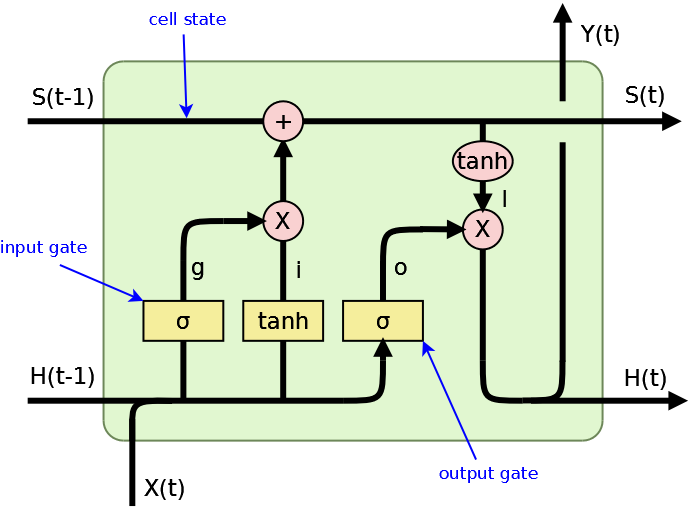
\includegraphics[scale=0.2]{images/LSTM_article_gates.png}
\caption{Différentes parties d'une cellule LSTM}
\label{cellule LSTM gates}
\end{center}
\end{figure}

Le cell state S correspond à la mémoire de la cellule. Celle-ci subit peu de modification au cours du temps, correspondant à l'ajout d'information dans la mémoire.

Les sigmoides permettent d'obtenir des sorties comprises entre 0 et 1. On peut donc pondérer l'importance d'une valeur en la multipliant par la sortie d'une sigmoïde. Si la sortie de la sigmoide est proche de 1, cela signifie que l'on garde la valeur, en revanche, si celle-ci est proche de 0, on oublie la valeur calculée.

Ainsi on calcule un vecteur i à partir de l'entrée et de la sortie précédente à l'aide d'une couche de tanh. Puis, on le multiplie terme à terme par le vecteur de sortie g d'une couche de sigmoides appelée input gate afin de sélectionner les informations que l'on souhaite conserver. Enfin, on ajoute ces informations sélectionnées dans le cell state. 

La sortie de la cellule est obtenue à partir du cell state auquel on applique une tanh. Enfin, on sélectionne les informations que l'on veut garder en sortie à l'aide d'une couche de sigmoides appelée output gate appliquée à l'entrée.


En pratique, on n'est pas sûr qu'une cellule LSTM suive effectivement le principe décrit précédemment. Celui-ci est plutôt une illustration afin de comprendre de manière générale le fonctionnement des LSTM.

La structure d'une cellule LSTM n'est pas non figée. En effet, il est possible de l'adapter en ajoutant, enlevant certains éléments, gates. Par exemple, on peut ajouter une forget gate composée d'une couche de sigmoides au début de la cellule. On multiplie la sortie de cette forget gate afin de garder, supprimer, réduire certaines composantes du cell state. 

\break

Dans le cas d'une cellule LSTM, les équations de propagation sont simples à calculer. En effet, comme pour le graphe de calcul, les équations sont directement données par le schéma.

Pour la bakcpropagation du gradient, il est toutefois nécessaire de calculer les formules à utiliser dans l'algorithme. La figure \ref{cellule LSTM gradient} fait apparaître le gradient à chaque endroit de la cellule.

\begin{figure}[h!]
\begin{center}
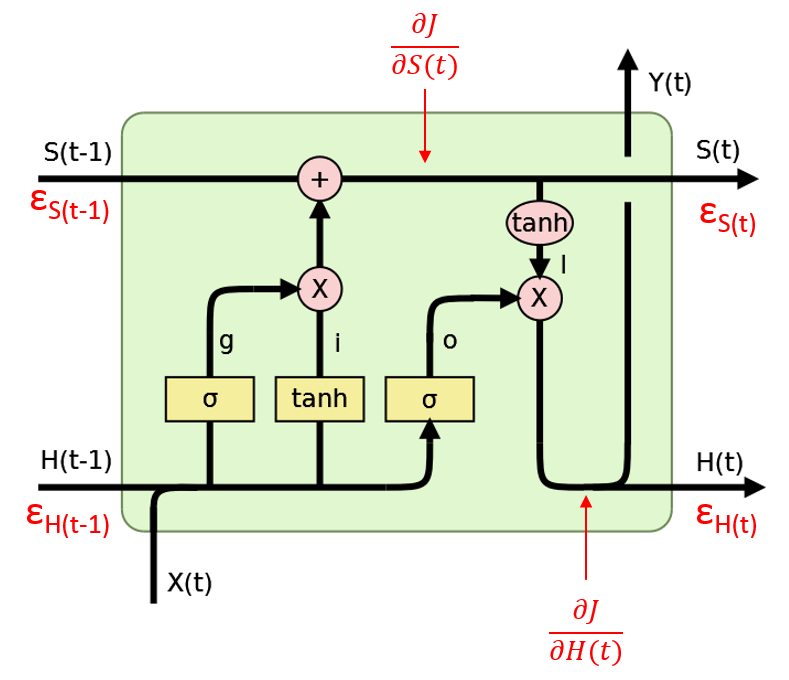
\includegraphics[scale=0.3]{images/LSTM_gradient.png}
\caption{Cellule LSTM}
\label{cellule LSTM gradient}
\end{center}
\end{figure}


En utilisant, BPTT pour rétropropager le gradient sur le graphe du LSTM déplié, on obtient les formules suivantes :

\begin{equation}
\varepsilon_{S(t-1)} = \frac{\partial J}{\partial S(t)} = \varepsilon_{S(t)} + F_{l}^{\prime}\text{diag}(o)\frac{\partial J}{\partial H(t)}
\end{equation}

\begin{equation}
\varepsilon_{H(t-1)} = \left((W_{g}^{T}F_{g}^{\prime}\text{diag}(i) + W_{i}^{T}F_{i}^{\prime}\text{diag}(g))\frac{\partial J}{\partial S(t)} + W_{o}^{T}F_{o}^{\prime}\text{diag}(l)\frac{\partial J}{\partial H(t)}\right)_{1,...,n}
\end{equation}

avec :

\[
F_{l}^{\prime} = \text{diag}((1 - l_{i}^{2})_{i=1,...,n})
\]

\[
F_{i}^{\prime} = \text{diag}((1 - i_{i}^{2})_{i=1,...,n})
\]

\[
F_{g}^{\prime} = \text{diag}((g_{i}(1 - g_{i}))_{i=1,...,n})
\]

\[
F_{o}^{\prime} = \text{diag}((o_{i}(1 - o_{i}))_{i=1,...,n})
\]


Il est alors possible de calculer le gradient relatif à chaque matrice de poids.

\begin{equation}
\frac{\partial J}{\partial W_{o}}=
\begin{pmatrix}
H(t-1) \\
x(t)
\end{pmatrix}
\left(F_{o}^{\prime}\text{diag}(l)\frac{\partial J}{\partial H(t)}\right)^{T}
\end{equation}

\begin{equation}
\frac{\partial J}{\partial W_{i}}=
\begin{pmatrix}
H(t-1) \\
x(t)
\end{pmatrix}
\left(F_{i}^{\prime}\text{diag}(g)\frac{\partial J}{\partial S(t)}\right)^{T}
\end{equation}

\begin{equation}
\frac{\partial J}{\partial W_{g}}=
\begin{pmatrix}
H(t-1) \\
x(t)
\end{pmatrix}
\left(F_{g}^{\prime}\text{diag}(i)\frac{\partial J}{\partial S(t)}\right)^{T}
\end{equation}

On rétropropage le gradient dans tout le graphe déplié avec les formules précédentes. Celui-ci est à chaque fois accumulé au niveau des poids. Les poids $W_{o}$, $W_{i}$ et $W_{g}$ sont alors mis à jour avec la formule :

\begin{equation}
W = W - \eta \sum{\frac{\partial J}{\partial W}}
\end{equation} 

\section{Implémentation}
\section{Résultats}
\section{Autres applications}

\end{document}
